\documentclass[sigconf,nonacm]{acmart}

%% Enable subfigures
\usepackage{subfigure}
%% Enable numbers in scientific format.
\usepackage{siunitx}
%% Enable enumerate start from.
\usepackage{enumitem}

%% Enable theorems
\newtheorem{theorem}{Theorem}[section]
\newtheorem{lemma}[theorem]{Lemma}

%% Enable algorithms
\usepackage{algorithm}
\usepackage[noend]{algpseudocode}
\let\ReturnInline\Return
\renewcommand{\Return}{\State\ReturnInline}
\algrenewcommand\algorithmicrequire{$\rhd$}
\algrenewcommand\algorithmicensure{$\square$}

%% Fonts used in the template cannot be substituted; margin 
%% adjustments are not allowed.
\AtBeginDocument{%
  \providecommand\BibTeX{{%
    \normalfont B\kern-0.5em{\scshape i\kern-0.25em b}\kern-0.8em\TeX}}}

%% Rights management information.
\setcopyright{acmcopyright}
\copyrightyear{2018}
\acmYear{2018}
\acmDOI{XXXXXXX.XXXXXXX}

%% These commands are for a PROCEEDINGS abstract or paper.
\acmConference[Conference acronym 'XX]{Make sure to enter the correct
  conference title from your rights confirmation emai}{June 03--05,
  2018}{Woodstock, NY}
%% Title of the proceedings is different from ``Proceedings of ...''?
% \acmBooktitle{Woodstock '18: ACM Symposium on Neural Gaze Detection,
%  June 03--05, 2018, Woodstock, NY} 
% \acmPrice{15.00}
% \acmISBN{978-1-4503-XXXX-X/18/06}

%% Submission ID.
% \acmSubmissionID{123-A56-BU3}

%% Use the "author year" style of citations and references?
% \citestyle{acmauthoryear}

%% Message
\newcommand{\kk}[1]{{{\color{red} #1}}}
\newcommand{\ds}[1]{{{\color{blue} #1}}}
\newcommand{\su}[1]{{{\color{green} #1}}}

%% Ignore block
\newcommand{\ignore}[1]{}

%% Macros
\newcommand{\Lou}{\textit{Louvain}}
\newcommand{\Sta}{\textit{Static}}




\begin{document}

%% Full title of the paper.
\title[GVE-Leiden: Fast Leiden Algorithm for Community Detection in Shared Memory Setting]{GVE-Leiden: Fast Leiden Algorithm for \\Community Detection in Shared Memory Setting}

%% Short title to be used in page headers (optional).
% \title[short title]{full title}
% \subtitle{Something other than the title}

%% Authors and their affiliations.
\author{Subhajit Sahu}
\email{subhajit.sahu@research.iiit.ac.in}
\affiliation{%
  \institution{IIIT Hyderabad}
  \streetaddress{Professor CR Rao Rd, Gachibowli}
  \city{Hyderabad}
  \state{Telangana}
  \country{India}
  \postcode{500032}
}

%% Concise author list in page headers.
%\renewcommand{\shortauthors}{Sahu, Kothapalli, and Banerjee, et al.}

%% Show page numbers.
\settopmatter{printfolios=true}

%% Short summary of the work to be presented in the article.
\begin{abstract}
Community detection is the problem of identifying natural divisions in networks. Efficient parallel algorithms for identifying such divisions is critical in a number of applications, where the size of datasets have reached significant scales. This technical report presents one of the most efficient implementations of the Leiden algorithm, a high quality community detection method. On a server equipped with dual 16-core Intel Xeon Gold 6226R processors, our Leiden implementation, which we term as GVE-Leiden, outperforms the original Leiden, igraph Leiden, NetworKit Leiden, and cuGraph Leiden (running on NVIDIA A100 GPU) by $436\times$, $104\times$, $8.2\times$, and $3.0\times$ respectively --- achieving a processing rate of $403 M$ edges/s on a $3.8 B$ edge graph. In addition, GVE-Leiden improves performance at an average rate of $1.6\times$ for every doubling of threads.
\end{abstract}

%% The code below is generated by the tool at http://dl.acm.org/ccs.cfm.
\begin{CCSXML}
<ccs2012>
<concept>
<concept_id>10003752.10003809.10010170</concept_id>
<concept_desc>Theory of computation~Parallel algorithms</concept_desc>
<concept_significance>500</concept_significance>
</concept>
<concept>
<concept_id>10003752.10003809.10003635</concept_id>
<concept_desc>Theory of computation~Graph algorithms analysis</concept_desc>
<concept_significance>500</concept_significance>
</concept>
</ccs2012>
\end{CCSXML}

% \ccsdesc[500]{Theory of computation~Parallel algorithms}
% \ccsdesc[500]{Theory of computation~Graph algorithms analysis}

%% Pick words that accurately describe the work being presented.
\keywords{Community detection, Parallel Leiden implementation}

% \received{20 February 2007}
% \received[revised]{12 March 2009}
% \received[accepted]{5 June 2009}



%% Process the author and title information.
\maketitle

\section{Introduction}
\label{sec:introduction}
Community detection\ignore{, also know as clustering,} is the problem of uncovering the underlying structure of complex networks, i.e., identifying groups of vertices that exhibit dense internal connections but sparse connections with the rest of the network, in an unsupervised manner. It is an NP-hard problem with numerous applications in domains such as drug discovery, protein annotation, topic discovery, anomaly detection, and criminal identification. Communities identified are intrinsic when based on network topology alone, and are disjoint when each vertex belongs to only one community \cite{com-gregory10}.\ignore{One of the difficulties in the community detection problem is the lack of apriori knowledge on the number and size distribution of communities \cite{com-blondel08}.} The \textit{Louvain} method \cite{com-blondel08} is a popular heuristic-based approach for community detection, with the modularity metric \cite{com-newman06} being used to measure the quality of communities identified.

In recent years, the collection of data and the relationships among them, represented as graphs, have reached unmatched levels. This has necessitated the design of efficient parallel algorithms for community detection on large networks. The multicore/shared memory setting is crucial for community detection due to its energy efficiency and the prevalence of hardware with extensive DRAM sizes.\ignore{Optimizing parallel community detection algorithms for modern hardware architectures can yield notable performance benefits and competitive advantages across applications.} However, many of the current algorithms for community detection are challenging to parallelize due to their irregular and inherently sequential nature \cite{com-halappanavar17}, in addition to the complexities of handling concurrency, optimizing data access, reducing contention, minimizing load imbalance. Existing studies on Louvain propose algorithmic optimizations and parallelization techniques, but do not address optimization for the aggregation phase of the Louvain algorithm, which emerges as a bottleneck after the local-moving phase of the algorithm has been optimized. Moreover, these optimization techniques are scattered over a number of papers, making it difficult for a reader to get a grip over them.


%% Introduction for Leiden algorithm
Community detection in graphs is a well-studied problem, which involves finding subsets of nodes that exhibit higher connectivity among themselves than with the rest of the network. The obtained communities shed light on the organization and functionality of the network. Community detection has applications in topic discovery, protein annotation, recommendation systems, and targeted advertising \cite{com-gregory10}.

The \textit{Louvain} algorithm \cite{com-blondel08} has been pivotal in community detection. It employs a two-phase approach, comprising a local-moving phase and an aggregation phase, to iteratively optimize the modularity metric --- a measure of community quality. Despite its popularity, \textit{Louvain} has been observed to produce badly connected communities --- even internally-disconnected communities \cite{com-traag19}.

In response to this, \textit{Leiden} algorithm has been proposed as an improvement over \textit{Louvain}. It introduces an additional refinement phase between the local-moving and aggregation phases. The refinement phase allows nodes to explore and potentially form sub-communities within the communities identified during the local-moving phase. This enables \textit{Leiden} to identify well-connected communities \cite{com-traag19}.

However, applying the original \textit{Leiden} algorithm to massive graphs has raised computational bottlenecks, mainly due to its inherently sequential nature. In contexts where scalability is paramount, the development of an optimized parallel \textit{Leiden} algorithm becomes imperative. This poster addresses precisely this challenge by presenting a parallel implementation of \textit{Leiden} \kk{say Leiden algorithm. not just Leiden}, targeting both quality and efficiency.




\subsection{Our Contributions}

This report introduces GVE-Leiden, an optimized parallel implementation of Leiden\footnote{https://github.com/puzzlef/leiden-communities-openmp} for shared memory multicores. On a machine with two 16-core Intel Xeon Gold 6226R processors, GVE-Leiden outperforms Vite, Grappolo, and NetworKit Louvain by $50\times$, $22\times$, and $20\times$ respectively, achieving a processing rate of $560 M$ edges/s on a $3.8 B$ edge graph. With doubling of threads, GVE-Leiden exhibits an average performance scaling of $1.6\times$.

This poster presents an optimized parallel version of the \textit{Leiden} algorithm for community detection. Our implementation can identify communities in a large undirected web graph with $1.9$ billion edges in just $10$ seconds using a single 64-core CPU. When compared to our optimized parallel \textit{Louvain} implementation, \textit{Leiden} achieves a $20$-fold reduction in disconnected communities, slightly higher net modularity, and only a $26\%$ drop in performance. This makes \textit{Leiden} an attractive choice for community detection on massive graphs.



%% - Use --- for a dash.
%% - Use ``camera-ready'' for quotes.
%% - Use {\itshape very} or \textit{very} for italicized text.
%% - Use \verb|acmart| or {\verb|acmart|} for mono-spaced text.
%% - Use \url{https://capitalizemytitle.com/} for URLs.
%% - Use {\bfseries Do not modify this document.} for important boldface details.
%% - Use \ref{fig:name} for referencing.

%% For a block of pre-formatted text: 
% \begin{verbatim}
%   \renewcommand{\shortauthors}{McCartney, et al.}
% \end{verbatim}

%% For a list of items:
% \begin{itemize}
% \item the ``ACM Reference Format'' text on the first page.
% \item the ``rights management'' text on the first page.
% \item the conference information in the page header(s).
% \end{itemize}

%% For a table:
% \begin{table}
%   \caption{Frequency of Special Characters}
%   \label{tab:freq}
%   \begin{tabular}{ccl}
%     \toprule
%     Non-English or Math&Frequency&Comments\\
%     \midrule
%     \O & 1 in 1,000& For Swedish names\\
%     $\pi$ & 1 in 5& Common in math\\
%     \$ & 4 in 5 & Used in business\\
%     $\Psi^2_1$ & 1 in 40,000& Unexplained usage\\
%   \bottomrule
% \end{tabular}
% \end{table}

%% For a full-width table:
% \begin{table*}
%   \caption{Some Typical Commands}
%   \label{tab:commands}
%   \begin{tabular}{ccl}
%     \toprule
%     Command &A Number & Comments\\
%     \midrule
%     \texttt{{\char'134}author} & 100& Author \\
%     \texttt{{\char'134}table}& 300 & For tables\\
%     \texttt{{\char'134}table*}& 400& For wider tables\\
%     \bottomrule
%   \end{tabular}
% \end{table*}


%% For inline math:
% \begin{math}
%   \lim_{n\rightarrow \infty}x=0
% \end{math},

%% For a numbered equation:
% \begin{equation}
%   \lim_{n\rightarrow \infty}x=0
% \end{equation}

%% For an unnumbered equation:
% \begin{displaymath}
%   \sum_{i=0}^{\infty} x + 1
% \end{displaymath}

%% For a figure:
% \begin{figure}[h]
%   \centering
%   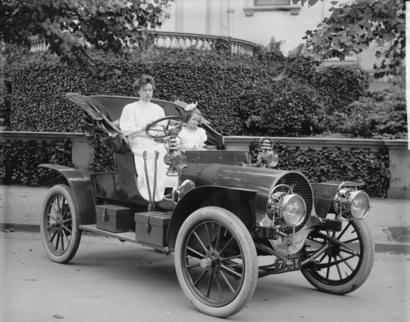
\includegraphics[width=\linewidth]{inc/sample-franklin}
%   \caption{1907 Franklin Model D roadster. Photograph by Harris \&
%     Ewing, Inc. [Public domain], via Wikimedia
%     Commons. (\url{https://goo.gl/VLCRBB}).}
%   \Description{A woman and a girl in white dresses sit in an open car.}
% \end{figure}

%% For a teaser figure.
% \begin{teaserfigure}
%   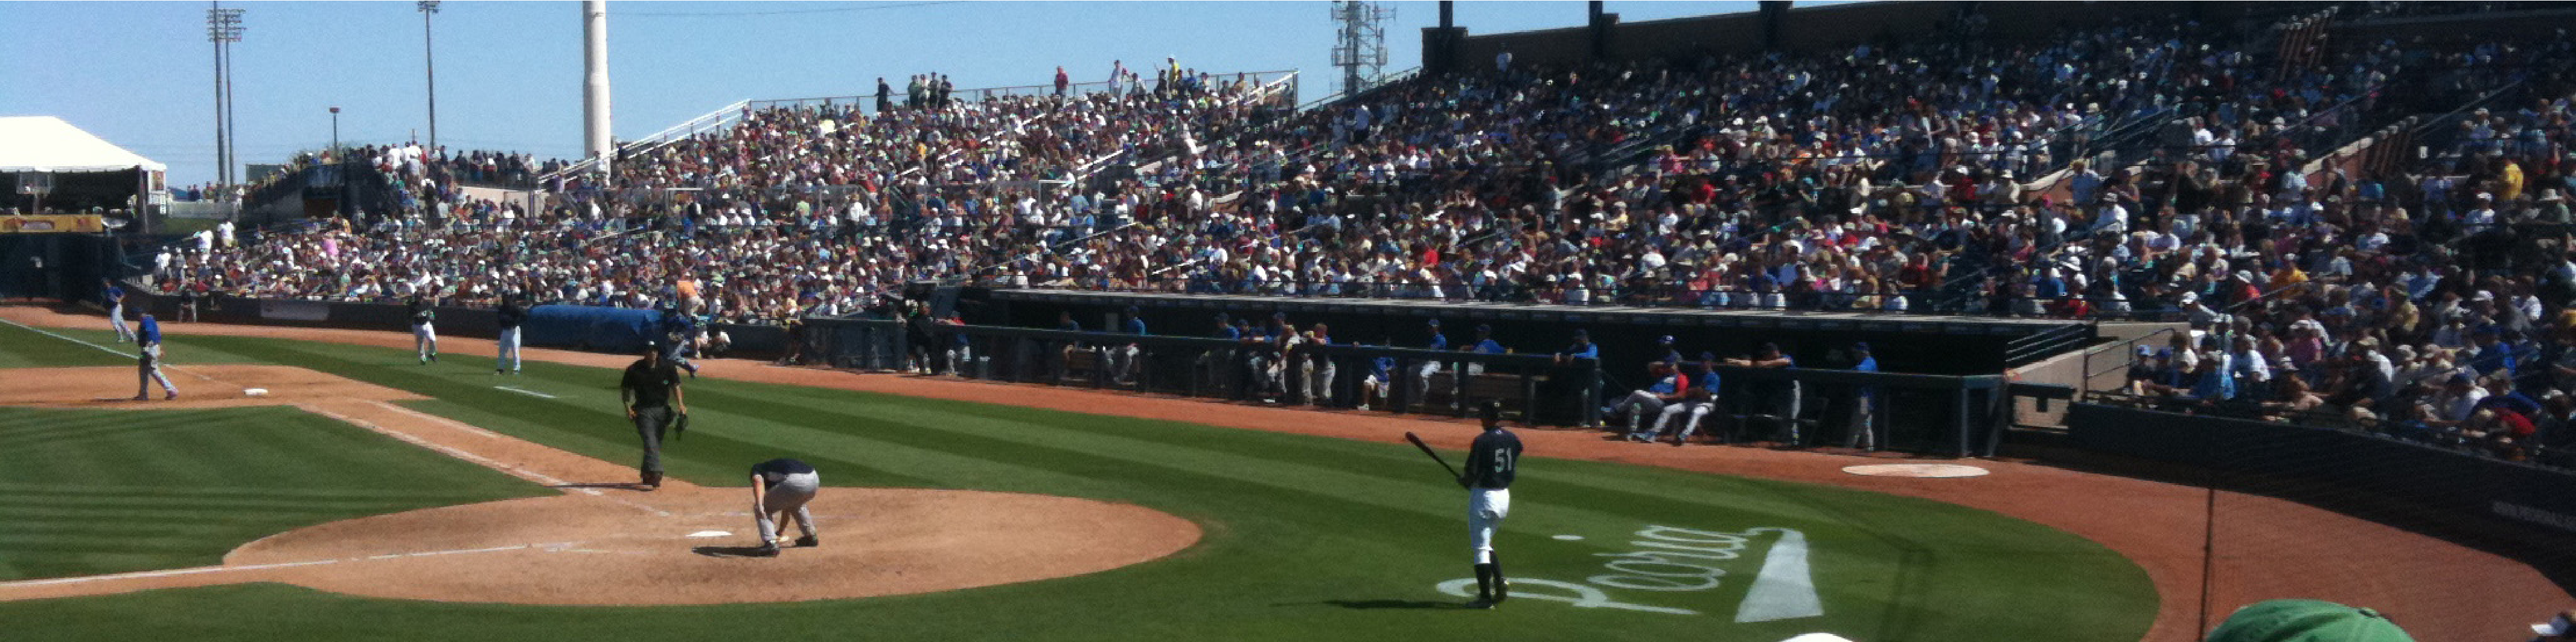
\includegraphics[width=\textwidth]{sampleteaser}
%   \caption{figure caption}
%   \Description{figure description}
% \end{teaserfigure}


\section{Related work}
\label{sec:related}
The \textit{Louvain} method is a greedy modularity-optimization based community detection algorithm, and is introduced by Blondel et al. from the University of Louvain \cite{com-blondel08}. It identifies communities with resulting high modularity, and is thus widely favored \cite{com-lancichinetti09}. Algorithmic improvements proposed for the original algorithm include early pruning of non-promising candidates (leaf vertices) \cite{com-ryu16, com-halappanavar17, com-zhang21, com-you22}, attempting local move only on likely vertices \cite{com-ryu16, com-ozaki16, com-zhang21, com-shi21}, ordering of vertices based on node importance \cite{com-aldabobi22}, moving nodes to a random neighbor community \cite{com-traag15}, threshold scaling \cite{com-lu15, com-naim17, com-halappanavar17}, threshold cycling \cite{com-ghosh18}, subnetwork refinement \cite{com-waltman13, com-traag19}, multilevel refinement \cite{com-rotta11, com-gach14, com-shi21}, and early termination \cite{com-ghosh18}.

To parallelize the Louvain algorithm, a number of strategies have been attempted. These include using heuristics to break the sequential barrier \cite{com-lu15}, ordering vertices via graph coloring \cite{com-halappanavar17}, performing iterations asynchronously \cite{com-que15, com-shi21}, using adaptive parallel thread assignment \cite{com-fazlali17, com-naim17, com-sattar19, com-mohammadi20}, parallelizing the costly first iteration \cite{com-wickramaarachchi14}, using vector based hashtables \cite{com-halappanavar17}, and using sort-reduce instead of hashing \cite{com-cheong13}\ignore{, using simple partitions based of vertex ids \cite{com-cheong13, com-ghosh18}, and identifying and moving ghost/doubtful vertices \cite{com-zeng15, com-que15, com-bhowmik19, com-bhowmick22}}. Platforms used range from an AMD multicore system \cite{com-fazlali17}, and Intel’s Knight's Landing, Haswell \cite{com-gheibi20}, SkylakeX, and Cascade Lake \cite{part-hossain21}. Other approaches include the use of MapReduce in a BigData batch processing framework \cite{com-zeitz17}. It should however be noted though that community detection methods such as the Louvain that rely on modularity maximization are known to suffer from resolution limit problem. This prevents identification of communities of certain sizes \cite{com-ghosh19}.

A few open source implementations and software packages have been developed for community detection. Vite \cite{ghosh2018scalable} is a distributed memory parallel implementation of the Louvain method that incorporates several heuristics to enhance performance while maintaining solution quality, while Grappolo \cite{com-halappanavar17} is a shared memory parallel implementation. NetworKit \cite{staudt2016networkit} is a software package designed for analyzing the structural aspects of graph data sets with billions of connections. It is implemented as a hybrid with C++ kernels and a Python frontend, and includes a parallel implementation of the Louvain algorithm.


%% Related work on Leiden algorithm

I see two thesis by Fabian, Karlsruhe Institute of Technology and Magnus, University of Bergen. Fabian uses global queues and for vertex pruning, and vertex and community locking for updating communities, which is likely to be less efficient. Magnus uses the same approach as Fabien. On europe graph their algorithm takes 60-70s with 64 threads (on a 128 core system).


%% Some related work for community detection

I dont know what a semiring is but this paper by cuGraphs authors suggest it is useful for community detection.
"In addition to embedding techniques, our primitive enables many important clustering and community detection algorithms, including k-means, k-medioids, mean-shift clustering, Louvain, Leiden, OPTICS, DBSCAN / HDBSCAN, Single- and complete-linkage agglomerative clustering, and Laplacian eigenmaps."
https://arxiv.org/abs/2104.06357


In the Parallel Heuristics for Scalable Community Detection, the authors describe the issues with trying to parallelize: possibility of negative gain, community swapping, stuck in local optima. Heuristics like minimum labeling, vertex coloring, and vertex following. Implementation is in OpenMP C++ and they used STL map for communities each vertex is connected to (i was trying this with pre-counting instead which could be faster). They compare using modularity score mostly. Specificity, Sensitivity, Overlap quality, and Rand index are difficult to calculate for large graphs (based on true positive, false positive, FN, TN). Modularity gain thresholds $10^-2$, $10^-4$. Comparision is also with label propagation based parallelization (PLM). There is also another community detection method called Clauset Newman Moore (CNM) which is agglomerative (cluster hierarchies tend to be more meaningful).
https://arxiv.org/pdf/1410.1237.pdf


%% More related work for community detection

I found one paper by Prof. L. Dhulipala "Scalable community detection via Parallel Correlation Clustering". They write about (static) Louvain algorithm using LambdaCC objective (instead of modularity). They explore three optimizations for the Louvain algorithm:
- They find asynchronous (ordered) Louvain performs well (quality and speed due to symmetry breaking).
(I observe the same in experiments too)
- They filter which vertices to consider moving in the next iteration (instead of all).
(This is similar to Dynamic Frontier but applied to static algorithm)
- They do an additional refinement after clustering (this minimizes bad clusters).
(This is similar to refinement phase in Leiden algorithm)


They use graphs varying from 1M to 1.8B edges, and do weak and strong scaling experiments.



\section{Preliminaries}
\label{sec:preliminaries}
Consider an undirected graph $G(V, E, w)$ with $V$ representing the set of vertices, $E$ the set of edges, and $w_{ij} = w_{ji}$ denoting the weight associated with each edge. In the case of an unweighted graph, we assume unit weight for each edge ($w_{ij} = 1$). Additionally, the neighbors of a vertex $i$ are denoted as $J_i = \{j\ |\ (i, j) \in E\}$, the weighted degree of each vertex as $K_i = \sum_{j \in J_i} w_{ij}$, the total number of vertices as $N = |V|$, the total number of edges as $M = |E|$, and the sum of edge weights in the undirected graph as $m = \sum_{i, j \in V} w_{ij}/2$.




\subsection{Community detection}

Disjoint community detection is the process of identifying a community membership mapping, $C: V \rightarrow \Gamma$, where each vertex $i \in V$ is assigned a community-id $c \in \Gamma$, where $\Gamma$ is the set of community-ids. We denote the vertices of a community $c \in \Gamma$ as $V_c$, and the community that a vertex $i$ belongs to as $C_i$. Further, we denote the neighbors of vertex $i$ belonging to a community $c$ as $J_{i \rightarrow c} = \{j\ |\ j \in J_i\ and\ C_j = c\}$, the sum of those edge weights as $K_{i \rightarrow c} = \sum_{j \in J_{i \rightarrow c}} w_{ij}$, the sum of weights of edges within a community $c$ as $\sigma_c = \sum_{(i, j) \in E\ and\ C_i = C_j = c} w_{ij}$, and the total edge weight of a community $c$ as $\Sigma_c = \sum_{(i, j) \in E\ and\ C_i = c} w_{ij}$ \cite{com-leskovec21}.




\subsection{Modularity}

Modularity serves as a\ignore{fitness} metric for assessing the quality of communities identified by heuristic-based community detection algorithms. It is computed as the difference between the fraction of edges within communities and the expected fraction if edges were randomly distributed, yielding a range of $[-0.5, 1]$ where higher values indicate better results \cite{com-brandes07}.\ignore{The optimization of this metric theoretically leads to the optimal grouping \cite{com-newman04, com-traag11}.} The modularity $Q$ of identified communities is determined using Equation \ref{eq:modularity}, where $\delta$ represents the Kronecker delta function ($\delta (x,y)=1$ if $x=y$, $0$ otherwise). The \textit{delta modularity} of moving a vertex $i$ from community $d$ to community $c$, denoted as $\Delta Q_{i: d \rightarrow c}$, can be computed using Equation \ref{eq:delta-modularity}.

\begin{equation}
\label{eq:modularity}
  Q
  = \frac{1}{2m} \sum_{(i, j) \in E} \left[w_{ij} - \frac{K_i K_j}{2m}\right] \delta(C_i, C_j)
  = \sum_{c \in \Gamma} \left[\frac{\sigma_c}{2m} - \left(\frac{\Sigma_c}{2m}\right)^2\right]
\end{equation}

\begin{equation}
\label{eq:delta-modularity}
  \Delta Q_{i: d \rightarrow c}
  = \frac{1}{m} (K_{i \rightarrow c} - K_{i \rightarrow d}) - \frac{K_i}{2m^2} (K_i + \Sigma_c - \Sigma_d)
\end{equation}




\subsection{Louvain algorithm}
\label{sec:about-louvain}

The Louvain method \cite{com-blondel08} is a modularity optimization based agglomerative algorithm for identifying high quality disjoint communities in large networks. It has a time complexity of $O (L |E|)$ (with $L$ being the total number of iterations performed), and a space complexity of $O(|V| + |E|)$ \cite{com-lancichinetti09}. The algorithm consists of two phases: the \textit{local-moving phase}, where each vertex $i$ greedily decides to move to the community of one of its neighbors $j \in J_i$ that gives the greatest increase in modularity $\Delta Q_{i:C_i \rightarrow C_j}$ (using Equation \ref{eq:delta-modularity}), and the \textit{aggregation phase}, where all the vertices in a community are collapsed into a single super-vertex. These two phases make up one pass, which repeats until there is no further increase in modularity \cite{com-blondel08, com-leskovec21}. We observe that Louvain obtains high-quality communities, with $3.0 - 30\%$ higher modularity than that obtained by LPA, but requires $2.3 - 14\times$ longer to converge.


\section{Approach}
\label{sec:approach}
\subsection{Optimizations for Leiden algorithm}
\label{sec:leiden}

We extend our optimization techniques, originally designed for the Louvain method \cite{sahu2023gvelouvain}, to the Leiden algorithm. Specifically, we implement an \textit{asynchronous} version of the Leiden algorithm, allowing threads to operate independently on distinct sections of the graph. While this approach promotes faster convergence, it also introduces variability into the final result \cite{com-shi21}. To ensure efficient computations, we allocate a dedicated hashtable per thread. These hashtables serve two main purposes: they keep track of the delta-modularity associated with moving to each community connected to a vertex during the local-moving/refinement phases, and they record the total edge weight between super-vertices in the aggregation phase of the algorithm \cite{sahu2023gvelouvain}.

Our optimizations encompass several strategies, including utilizing OpenMP's \textit{dynamic} loop scheduling, capping the number of iterations per pass at $20$, employing a tolerance drop rate of $10$ (threshold scaling), initiating with a tolerance of $0.01$, using an aggregation tolerance of $0.8$ to avoid performing aggregations of minimal utility, implementing flag-based vertex pruning (instead of a queue-based one \cite{nguyenleiden}), utilizing parallel prefix sum, and using preallocated Compressed Sparse Row (CSR) data structures for identifying community vertices and storing the super-vertex graph during aggregation. Additionally, we employ fast collision-free per-thread hashtables, well separated in their memory addresses \cite{sahu2023gvelouvain}.

We attempt two approaches of the Leiden algorithm. One uses a \textit{greedy refinement phase} where vertices greedily optimize for delta-modularity (within their community bounds), while the other uses a \textit{randomized refinement phase} (using fast \textit{xorshift32} random number generators), where the likelihood of selection of a community to move to (by a vertex) is proportional to its delta-modularity, as originally proposed \cite{com-traag19}. Our results, shown in Figures \ref{fig:leidenopt-runtime} and \ref{fig:leidenopt-modularity}, indicate the \textit{greedy approach} performs the best on average, both in terms of runtime and modularity. We also try medium and heavy variants for both approaches, which disables threshold scaling and aggregation tolerance (including threshold scaling) respectively, However, we do not find them to perform well overall.\ignore{On \textit{europe\_osm} graph, our parallel Greedy-Leiden (which we from here on refer to simply as Leiden) runs $3\times$ faster than Nguyen \cite{nguyenleiden}.}

\ignore{We fixed a bug that caused the Leiden algorithm to fail in finding communities on road networks and kmer graphs. The issue was forgetting to reset the affected vertices flags before running the refinement phase.}

\begin{figure}[hbtp]
  \centering
  \subfigure{
    \label{fig:leidenopt-runtime--all}
    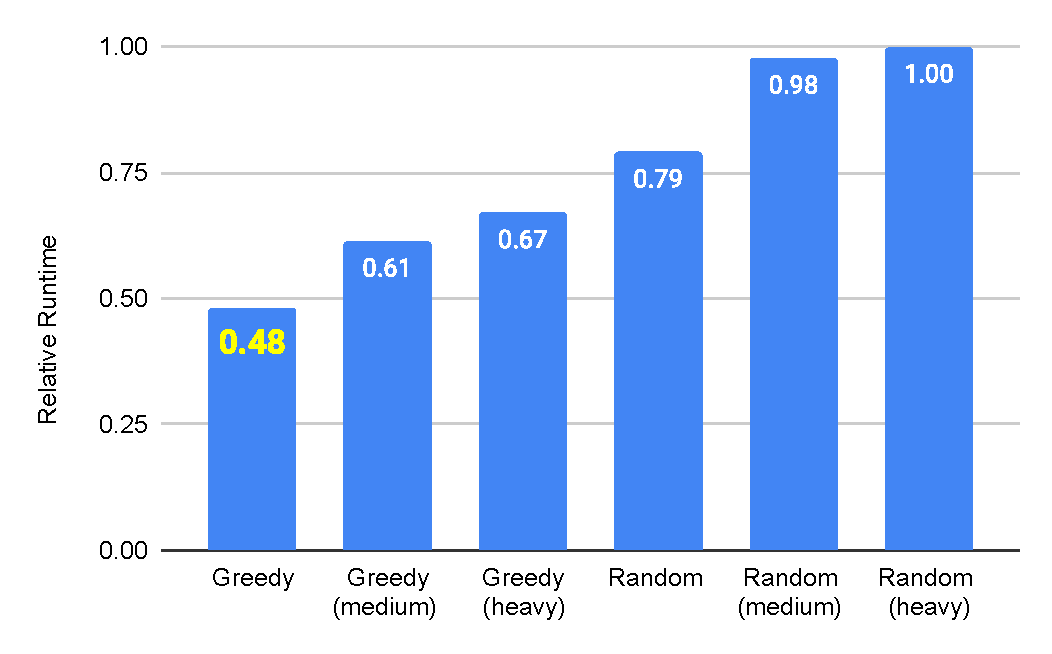
\includegraphics[width=0.98\linewidth]{out/leidenopt-runtime.pdf}
  } \\[-2ex]
  \caption{Average relative runtime for the \textit{greedy} and \textit{random} approaches (including \textit{medium} and \textit{heavy} variants) of parallel Leiden algorithm for all graphs in the dataset.}
  \label{fig:leidenopt-runtime}
\end{figure}

\begin{figure}[hbtp]
  \centering
  \subfigure{
    \label{fig:leidenopt-modularity--all}
    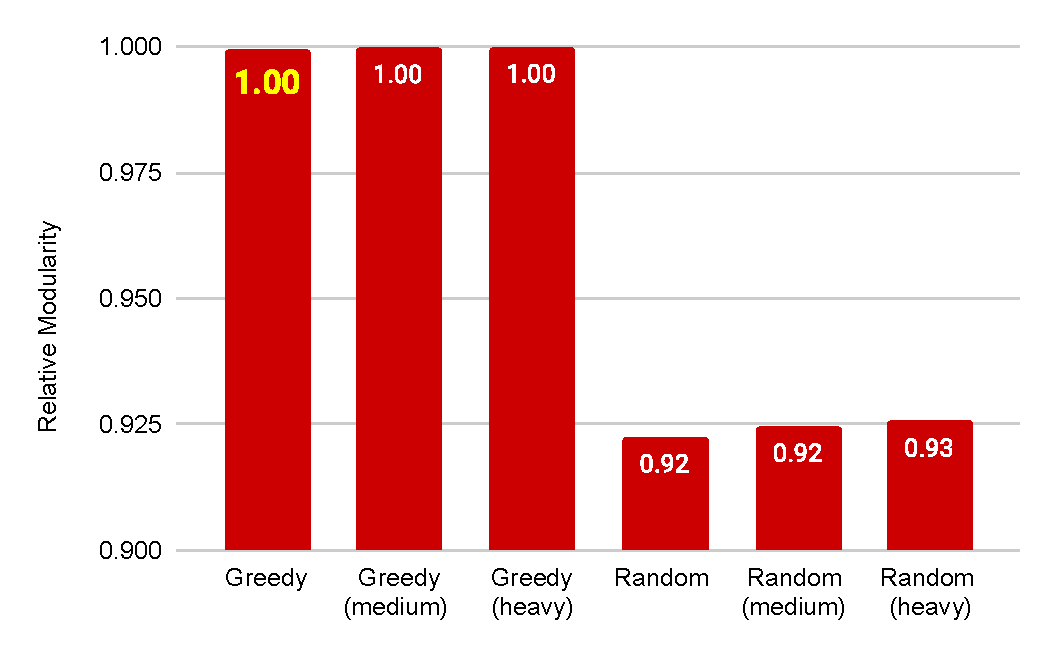
\includegraphics[width=0.98\linewidth]{out/leidenopt-modularity.pdf}
  } \\[-2ex]
  \caption{Average relative modularity for the \textit{greedy} and \textit{random} approaches (including \textit{medium} and \textit{heavy} variants) of parallel Leiden algorithm for all graphs in the dataset.}
  \label{fig:leidenopt-modularity}
\end{figure}

\begin{figure*}[hbtp]
  \centering
  \subfigure{
    \label{fig:leiden-pass--all}
    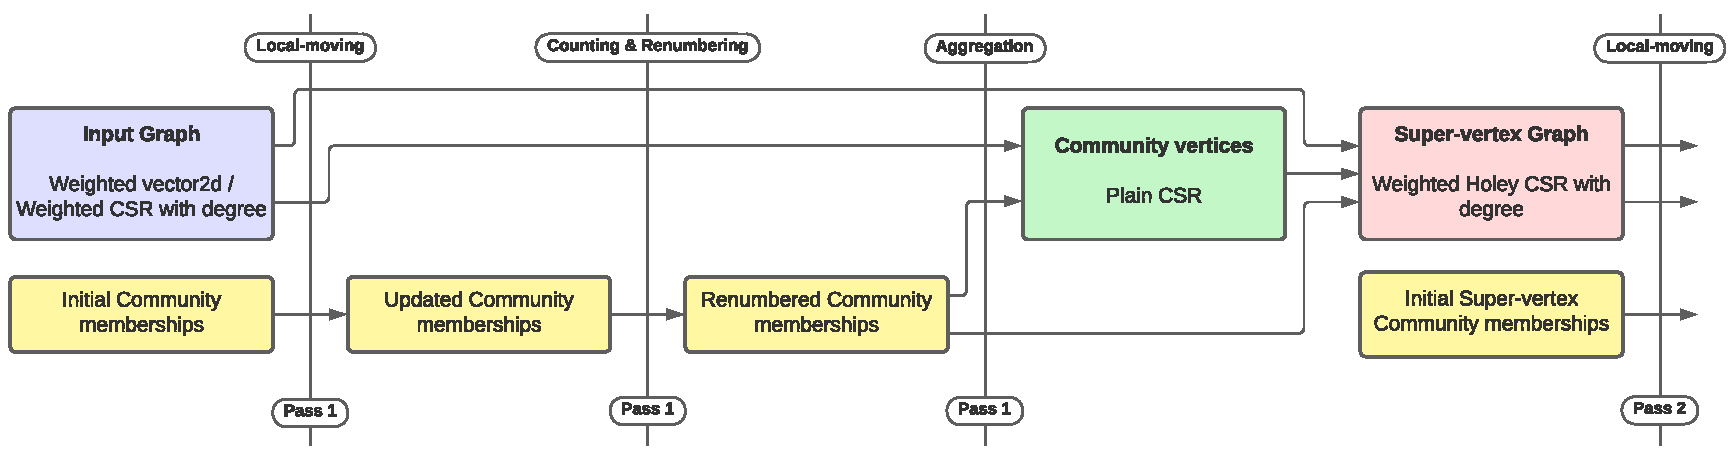
\includegraphics[width=0.98\linewidth]{out/leiden-pass.pdf}
  } \\[-2ex]
  \caption{A flow diagram illustrating the first pass of GVE-Leiden for either a Weighted 2D-vector-based or a Weighted CSR with degree-based input graph. In the local-moving phase, vertex community memberships are updated to obtain community bounds for the refinement phase, until the cumulative delta-modularity change across all vertices reaches a specified threshold. Then, in the refinement phase, the each vertex starts in a singleton community, and community memberships are updated similarly to the local-moving phase, with vertices changing communities within their bounds. These community memberships are then counted and renumbered. In the aggregation phase, community vertices in a CSR are first obtained. This is used to create the super-vertex graph stored in a Weighted Holey CSR with degree. Subsequent passes use a Weighted Holey CSR with degree and initial community memberships for super-vertices from the previous pass as input.}
  \label{fig:leiden-pass}
\end{figure*}





\subsection{Our optimized Leiden implementation}

We now explain the implementation of GVE-Leiden in Algorithms \ref{alg:leiden}, \ref{alg:leidenlm}, \ref{alg:leidenre}, and \ref{alg:leidenag}. A flow diagram illustrating the first pass of GVE-Leiden is shown in Figure \ref{fig:leiden-pass}.


\subsubsection{Main step of GVE-Leiden}

The main step of GVE-Leiden (\texttt{leiden()} function) is outlined in Algorithm \ref{alg:leiden}. It encompasses initialization, the local-moving phase, the refinement phase, and the aggregation phase. Here, the \texttt{leiden()} function accepts the input graph $G$, and returns the community membership $C$ of each vertex. In line \ref{alg:leiden--initialization}, we first initialize the community membership $C$ for each vertex in $G$, and perform passes of the Leiden algorithm, limited to $MAX\_PASSES$ (lines \ref{alg:leiden--passes-begin}-\ref{alg:leiden--passes-end}). During each pass, we initialize the total edge weight of each vertex $K'$, the total edge weight of each community $\Sigma'$, and the community membership $C'$ of each vertex in the current graph $G'$ (line \ref{alg:leiden--reset-weights}).

Subsequently, in line \ref{alg:leiden--local-move}, we perform the local-moving phase by invoking \texttt{leidenMove()} (Algorithm \ref{alg:leidenlm}), which optimizes community assignments. Following this, we set the \textit{community bound} of each vertex (for the refinement phase) as the community membership of each vertex just obtained, and reset the membership of each vertex, and the total weight of each community as singleton vertices in line \ref{alg:leiden--reset-again}. In line \ref{alg:leiden--refine}, the refinement phase is carried out by invoking \texttt{leidenRefine()} (Algorithm \ref{alg:leidenre}), which optimizes the community assignment of each vertex within its community bound. If either the local-moving or the refinement phase converged in a single iteration, global convergence is implied and we terminate the passes (line \ref{alg:leiden--globally-converged}). Further, if the drop in community count $|\Gamma|$ is marginal, we halt at the current pass (line \ref{alg:leiden--aggregation-tolerance}).

If convergence has not been achieved, we proceed to renumber communities (line \ref{alg:leiden--renumber}), update top-level community memberships $C$ with dendrogram lookup (line \ref{alg:leiden--lookup}), perform the aggregation phase by calling \texttt{leidenAggregate()} (Algorithm \ref{alg:leidenag}), and adjust the convergence threshold for subsequent passes, i.e., perform threshold scaling (line \ref{alg:leiden--threshold-scaling}). The next pass commences in line \ref{alg:leiden--passes-begin}. At the end of all passes, we perform a final update of the top-level community memberships $C$ with dendrogram lookup (line \ref{alg:leiden--lookup-last}), and return the top-level community membership $C$ of each vertex in $G$.

\begin{algorithm}[hbtp]
\caption{GVE-Leiden: Our parallel Leiden algorithm.}
\label{alg:leiden}
\begin{algorithmic}[1]
\Require{$G$: Input graph}
\Require{$C$: Community membership of each vertex}
\Require{$G'$: Input/super-vertex graph}
\Require{$C'$: Community membership of each vertex in $G'$}
\Require{$K'$: Total edge weight of each vertex}
\Require{$\Sigma'$: Total edge weight of each community}
\Ensure{$G'_{C'}$: Community vertices (CSR)}
\Ensure{$H_t$: Collision-free per-thread hashtable}
\Ensure{$l_i$, $l_j$: Number of iterations performed (per pass)}
\Ensure{$l_p$: Number of passes performed}
\Ensure{$\tau$: Per iteration tolerance}
\Ensure{$\tau_{agg}$: Aggregation tolerance}

\Statex

\Function{leiden}{$G$} \label{alg:leiden--begin}
  \State Vertex membership: $C \gets [0 .. |V|)$ \textbf{;} $G' \gets G$ \label{alg:leiden--initialization}
  \ForAll{$l_p \in [0 .. \text{\small{MAX\_PASSES}})$} \label{alg:leiden--passes-begin}
    \State $\Sigma' \gets K' \gets vertexWeights(G')$ \textbf{;} $C' \gets [0 .. |V'|)$ \label{alg:leiden--reset-weights}
    \State $l_i \gets leidenMove(G', C', K', \Sigma', \tau)$ \Comment{Alg. \ref{alg:leidenlm}} \label{alg:leiden--local-move}
    \State $C'_B \gets C'$ \textbf{;} $C' \gets [0 .. |V'|)$ \textbf{;} $\Sigma' \gets K'$ \label{alg:leiden--reset-again}
    \State $l_j \gets leidenRefine(G', C'_B, C', K', \Sigma', \tau)$ \Comment{Alg. \ref{alg:leidenre}} \label{alg:leiden--refine}
    \If{$l_i + l_j \le 1$} \textbf{break} \Comment{Globally converged?} \label{alg:leiden--globally-converged}
    \EndIf
    \State $|\Gamma|, |\Gamma_{old}| \gets$ Number of communities in $C$, $C'$
    \If{$|\Gamma|/|\Gamma_{old}| > \tau_{agg}$} \textbf{break} \Comment{Low shrink?} \label{alg:leiden--aggregation-tolerance}
    \EndIf
    \State $C' \gets$ Renumber communities in $C'$ \label{alg:leiden--renumber}
    \State $C \gets$ Lookup dendrogram using $C$ to $C'$ \label{alg:leiden--lookup}
    \State $G' \gets leidenAggregate(G', C')$ \Comment{Alg. \ref{alg:leidenag}} \label{alg:leiden--aggregate}
    \State $C' \gets$ Map $C'$ to $C'_B$ \Comment{Use move-based membership} \label{alg:leiden--useparent}
    \State $\tau \gets \tau / \text{\small{TOLERANCE\_DROP}}$ \Comment{Threshold scaling} \label{alg:leiden--threshold-scaling}
  \EndFor \label{alg:leiden--passes-end}
  \State $C \gets$ Lookup dendrogram using $C$ to $C'$ \label{alg:leiden--lookup-last}
  \Return{$C$} \label{alg:leiden--return}
\EndFunction \label{alg:leiden--end}
\end{algorithmic}
\end{algorithm}

\begin{algorithm}[hbtp]
\caption{Local-moving phase of GVE-Leiden.}
\label{alg:leidenlm}
\begin{algorithmic}[1]
\Require{$G'$: Input/super-vertex graph}
\Require{$C'$: Community membership of each vertex}
\Require{$K'$: Total edge weight of each vertex}
\Require{$\Sigma'$: Total edge weight of each community}
\Ensure{$G'_{C'}$: Community vertices (CSR)}
\Ensure{$H_t$: Collision-free per-thread hashtable}
\Ensure{$l_i$: Number of iterations performed}
\Ensure{$\tau$: Per iteration tolerance}

\Statex

\Function{leidenMove}{$G', C', K', \Sigma', \tau$} \label{alg:leidenlm--move-begin}
  \State Mark all vertices in $G'$ as unprocessed \label{alg:leidenlm--reset-affected}
  \ForAll{$l_i \in [0 .. \text{\small{MAX\_ITERATIONS}})$} \label{alg:leidenlm--iterations-begin}
    \State Total delta-modularity per iteration: $\Delta Q \gets 0$ \label{alg:leidenlm--init-deltaq}
    \ForAll{unprocessed $i \in V'$ \textbf{in parallel}} \label{alg:leidenlm--loop-vertices-begin}
      \State Mark $i$ as processed (prune) \label{alg:leidenlm--prune}
      \State $H_t \gets scanCommunities(\{\}, G', C', i, false)$ \label{alg:leidenlm--scan}
      \State $\rhd$ Use $H_t, K', \Sigma'$ to choose best community
      \State $c^* \gets$ Best community linked to $i$ in $G'$ \label{alg:leidenlm--best-community-begin}
      \State $\delta Q^* \gets$ Delta-modularity of moving $i$ to $c^*$ \label{alg:leidenlm--best-community-end}
      \If{$c^* = C'[i]$} \textbf{continue} \label{alg:leidenlm--best-community-same}
      \EndIf
      \State $\Sigma'[C'[i]] -= K'[i]$ \textbf{;} $\Sigma'[c^*] += K'[i]$ \textbf{atomic} \label{alg:leidenlm--perform-move-begin}
      \State $C'[i] \gets c^*$ \textbf{;} $\Delta Q \gets \Delta Q + \delta Q^*$ \label{alg:leidenlm--perform-move-end}
      \State Mark neighbors of $i$ as unprocessed \label{alg:leidenlm--remark}
    \EndFor \label{alg:leidenlm--loop-vertices-end}
    \If{$\Delta Q \le \tau$} \textbf{break} \Comment{Locally converged?} \label{alg:leidenlm--locally-converged}
    \EndIf
  \EndFor \label{alg:leidenlm--iterations-end}
  \Return{$l_i$} \label{alg:leidenlm--return}
\EndFunction \label{alg:leidenlm--move-end}

\Statex

\Function{scanCommunities}{$H_t, G', C', i, self$}
  \ForAll{$(j, w) \in G'.edges(i)$}
    \If{\textbf{not} $self$ \textbf{and} $i = j$} \textbf{continue}
    \EndIf
    \State $H_t[C'[j]] \gets H_t[C'[j]] + w$
  \EndFor
  \Return{$H_t$}
\EndFunction
\end{algorithmic}
\end{algorithm}

\begin{algorithm}[hbtp]
\caption{Refinement phase of GVE-Leiden.}
\label{alg:leidenre}
\begin{algorithmic}[1]
\Require{$G'$: Input/super-vertex graph}
\Require{$C'$: Community membership of each vertex}
\Require{$K'$: Total edge weight of each vertex}
\Require{$\Sigma'$: Total edge weight of each community}
\Ensure{$G'_{C'}$: Community vertices (CSR)}
\Ensure{$H_t$: Collision-free per-thread hashtable}
\Ensure{$\tau$: Per iteration tolerance}

\Statex

\Function{leidenRefine}{$G', C'_B, C', K', \Sigma', \tau$} \label{alg:leidenre--move-begin}
  \ForAll{$i \in V'$ \textbf{in parallel}} \label{alg:leidenre--loop-vertices-begin}
    \If{$\Sigma'[C'[i]] \neq K'[i]$} \textbf{continue} \label{alg:leidenre--check-isolated}
    \EndIf
    \State $H_t \gets scanBounded(\{\}, G', C'_B, C', i, false)$ \label{alg:leidenre--scan}
    \State $\rhd$ Use $H_t, K', \Sigma'$ to choose best community
    \State $c^* \gets$ Best community linked to $i$ in $G'$ within $C'_B$ \label{alg:leidenre--best-community-begin}
    \State $\delta Q^* \gets$ Delta-modularity of moving $i$ to $c^*$ \label{alg:leidenre--best-community-end}
    \If{$c^* = C'[i]$} \textbf{continue} \label{alg:leidenre--best-community-same}
    \EndIf
    \If{$atomicCAS(\Sigma'[C'[i]], 0) = K'[C'[i]]$} \label{alg:leidenre--perform-move-begin}
      \State $\Sigma'[c^*] += K'[i]$ \textbf{atomically}
      \State $C'[i] \gets c^*$ \label{alg:leidenre--perform-move-end}
    \EndIf
  \EndFor \label{alg:leidenre--loop-vertices-end}
\EndFunction \label{alg:leidenre--move-end}

\Statex

\Function{scanBounded}{$H_t, G', C'_B, C', i, self$}
  \ForAll{$(j, w) \in G'.edges(i)$}
    \If{\textbf{not} $self$ \textbf{and} $i = j$} \textbf{continue}
    \EndIf
    \If{$C'_B[i] \neq C'_B[j]$} \textbf{continue}
    \EndIf
    \State $H_t[C'[j]] \gets H_t[C'[j]] + w$
  \EndFor
  \Return{$H_t$}
\EndFunction

\Statex

\Function{atomicCAS}{$pointer, old, new$}
  \State $\rhd$ Perform the following atomically
  \If{$pointer = old$} $pointer \gets new$ \textbf{;} \ReturnInline{$old$}
  \Else\ \ReturnInline{$pointer$}
  \EndIf
\EndFunction
\end{algorithmic}
\end{algorithm}

\begin{algorithm}[hbtp]
\caption{Aggregation phase of GVE-Leiden.}
\label{alg:leidenag}
\begin{algorithmic}[1]
\Require{$G'$: Input/super-vertex graph}
\Require{$C'$: Community membership of each vertex}
\Ensure{$G'_{C'}$: Community vertices (CSR)}
\Ensure{$G''$: Super-vertex graph (weighted CSR)}
\Ensure{$*.offsets$: Offsets array of a CSR graph}
\Ensure{$H_t$: Collision-free per-thread hashtable}

\Statex

\Function{leidenAggregate}{$G', C'$}
  \State $\rhd$ Obtain vertices belonging to each community
  \State $G'_{C'}.offsets \gets countCommunityVertices(G', C')$ \label{alg:leidenag--coff-begin}
  \State $G'_{C'}.offsets \gets exclusiveScan(G'_{C'}.offsets)$ \label{alg:leidenag--coff-end}
  \ForAll{$i \in V'$ \textbf{in parallel}} \label{alg:leidenag--comv-begin}
    \State Add edge $(C'[i], i)$ to CSR $G'_{C'}$ \textbf{atomically}
  \EndFor \label{alg:leidenag--comv-end}
  \State $\rhd$ Obtain super-vertex graph
  \State $G''.offsets \gets communityTotalDegree(G', C')$ \label{alg:leidenag--yoff-begin}
  \State $G''.offsets \gets exclusiveScan(G''.offsets)$ \label{alg:leidenag--yoff-end}
  \State $|\Gamma| \gets$ Number of communities in $C'$
  \ForAll{$c \in [0, |\Gamma|)$ \textbf{in parallel}} \label{alg:leidenag--y-begin}
    % \If{degree of $c$ in $G'_{C'} = 0$} \textbf{continue}
    % \EndIf
    \State $H_t \gets \{\}$
    \ForAll{$i \in G'_{C'}.edges(c)$}
      \State $H_t \gets scanCommunities(H_t, G', C', i, true)$
    \EndFor
    \ForAll{$(d, w) \in H_t$}
      \State Add edge $(c, d, w)$ to CSR $G''$ \textbf{atomically}
    \EndFor
  \EndFor \label{alg:leidenag--y-end}
  \Return $G''$ \label{alg:leidenag--return}
\EndFunction
\end{algorithmic}
\end{algorithm}



\subsubsection{Local-moving phase of GVE-Leiden}

The pseuodocode for the local-moving phase of GVE-Leiden is shown in Algorithm \ref{alg:leidenlm}, which iteratively moves vertices between communities to maximize modularity. Here, the \texttt{leidenMove()} function takes the current graph $G'$, community membership $C'$, total edge weight of each vertex $K'$ and each community $\Sigma'$, the iteration tolerance $\tau$ as input, and returns the number of iterations performed $l_i$.

Lines \ref{alg:leidenlm--iterations-begin}-\ref{alg:leidenlm--iterations-end} represent the main loop of the local-moving phase. In line \ref{alg:leidenlm--reset-affected}, we first mark all vertices as unprocessed. Then, in line \ref{alg:leidenlm--init-deltaq}, we initialize the total delta-modularity per iteration $\Delta Q$. Next, in lines \ref{alg:leidenlm--loop-vertices-begin}-\ref{alg:leidenlm--loop-vertices-end}, we iterate over unprocessed vertices in parallel. For each unprocessed vertex $i$, we mark $i$ as processed - vertex pruning (line \ref{alg:leidenlm--prune}), scan communities connected to $i$ - excluding self (line \ref{alg:leidenlm--scan}), determine the best community $c*$ to move $i$ to (line \ref{alg:leidenlm--best-community-begin}), and calculate the delta-modularity of moving $i$ to $c*$ (line \ref{alg:leidenlm--best-community-end}). We then update the community membership of $i$ (lines \ref{alg:leidenlm--perform-move-begin}-\ref{alg:leidenlm--perform-move-end}) and mark its neighbors as unprocessed (line \ref{alg:leidenlm--remark}) if a better community was found. In line \ref{alg:leidenlm--locally-converged}, we check if the local-moving phase has converged. If so, we break out of the loop (or if $MAX\_ITERATIONS$ is reached). At the end, in line \ref{alg:leidenlm--return}, we return the number of iterations performed $l_i$.


\subsubsection{Refinement phase of GVE-Leiden}

The pseuodocode for the refinement phase of GVE-Leiden is presented in Algorithm \ref{alg:leidenlm}. This is similar to the local-moving phase, but utilizes the obtained community membership of each vertex as a \textit{community bound}, where each vertex must choose to join the community of another vertex within its community bound.\ignore{Similar to the local-moving phase however, vertices iteratively move between communities to maximize modularity.} At the start of the refinement phase, the community membership of each vertex is reset, such that each vertex belongs to its own community. Here, the \texttt{leidenRefine()} function takes the current graph $G'$, the community bound of each vertex $C'_B$, the initial community membership $C'$ of each vertex, the total edge weight of each vertex $K'$, the initial total edge weight of each community $\Sigma'$, and the current per iteration tolerance $\tau$ as input, and returns the number of iterations performed $l_j$.

Lines \ref{alg:leidenre--iterations-begin}-\ref{alg:leidenre--iterations-end} represent the core of the refinement phase. First, we initialize all vertices as unprocessed (line \ref{alg:leidenre--reset-affected}). Subsequently, we initialize the per-iteration delta-modularity $\Delta Q$ (line \ref{alg:leidenre--init-deltaq}), and iterate over unprocessed vertices in parallel (lines \ref{alg:leidenre--loop-vertices-begin}-\ref{alg:leidenre--loop-vertices-end}). For each unprocessed vertex $i$, we prune $i$ (line \ref{alg:leidenre--prune}), scan communities connected to $i$ within the \textit{same community bound} - excluding self (line \ref{alg:leidenre--scan}), evaluate the best community $c*$ to move $i$ to (line \ref{alg:leidenre--best-community-begin}), and compute the delta-modularity of moving $i$ to $c*$ (line \ref{alg:leidenre--best-community-end}). If a better community was found, we update the community membership (lines \ref{alg:leidenre--perform-move-begin}-\ref{alg:leidenre--perform-move-end}) of $i$, and mark its neighbors as unprocessed (line \ref{alg:leidenre--remark}). In line \ref{alg:leidenre--locally-converged}, we check if the refinement phase has converged. If so, we stop iterating (or if $MAX\_ITERATIONS$ is reached). Finally, we return the number of iterations performed $l_j$ (line \ref{alg:leidenre--return}).

% For each vertex $i$, the algorithm performs vertex pruning (line \ref{alg:leidenre--prune}), scans communities connected to $i$ within the \textit{same community bound} (excluding self) in line \ref{alg:leidenre--scan}, determines the optimal community $c*$ for relocating $i$ (lines \ref{alg:leidenre--best-community-begin} to \ref{alg:leidenre--best-community-end}), calculates the delta-modularity of moving $i$ to $c*$, and updates the community membership of $i$ (lines \ref{alg:leidenre--perform-move-begin} to \ref{alg:leidenre--perform-move-end}). If a better community is identified, the neighbors of $i$ are marked as unprocessed (line \ref{alg:leidenre--remark}). Line \ref{alg:leidenre--locally-converged} checks for local convergence in the moving phase, and if achieved, the loop is terminated (or if the maximum number of iterations $MAX\_ITERATIONS$ is reached). Finally, line \ref{alg:leidenre--return} returns the count of iterations performed, denoted as $l_j$.

\begin{algorithm}[hbtp]
\caption{Finding disconnected communities in parallel.}
\label{alg:disconnected}
\begin{algorithmic}[1]
\Require{$G$: Input graph}
\Require{$C$: Community membership of each vertex}
\Ensure{$D$: Disconnected flag for each community}
\Ensure{$S$: Size of each community}
\Ensure{$f_{if}$: Perform BFS to vertex $j$ if condition satisfied}
\Ensure{$f_{do}$: Perform operation after each vertex is visited}
\Ensure{$reached$: Number of vertices reachable from $i$ to $i$'s community}
\Ensure{$work_t$: Work-list of current thread}

\Statex

\Function{disconnectedCommunities}{$G, C$} \label{alg:disconnected--begin}
  \State $D \gets \{\}$ \textbf{;} $vis \gets \{\}$ \label{alg:disconnected--init}
  \State $S \gets communitySizes(G, C)$ \label{alg:disconnected--sizes}
  \ForAll{\textbf{threads in parallel}} \label{alg:disconnected--threads-begin}
    \ForAll{$i \in V$} \label{alg:disconnected--loop-begin}
      \State $c \gets C[i]$ \textbf{;} $reached \gets 0$ \label{alg:disconnected--unreached}
      \State $\rhd$ Skip if community $c$ is empty, or
      \State $\rhd$ does not belong to work-list of current thread.
      \If{$S[c] = 0$ \textbf{or} $c \notin work_t$} \textbf{continue} \label{alg:disconnected--work}
      \EndIf
      \State $f_{if} \gets (j) \implies C[j] = c$
      \State $f_{do} \gets (j) \implies reached \gets reached + 1$
      \State $bfsVisitForEach(vis, G, i, f_{if}, f_{do})$ \label{alg:disconnected--bfs}
      \If{$reached < S[c]$} $D[c] \gets 1$ \label{alg:disconnected--mark}
      \EndIf
      \State $S[c] \gets 0$ \label{alg:disconnected--processed}
    \EndFor \label{alg:disconnected--loop-end}
  \EndFor \label{alg:disconnected--threads-end}
  \Return{$D$}
\EndFunction \label{alg:disconnected--end}
\end{algorithmic}
\end{algorithm}



\subsubsection{Aggregation phase of GVE-Leiden}

Finally, we show the psuedocode for the aggregation phase in Algorithm \ref{alg:leidenag}, where communities are aggregated into super-vertices in preparation for the next pass of the Leiden algorithm (which operates on the super-vertex graph). Here, the \texttt{leidenAggregate()} function takes the current graph $G'$ and the community membership $C'$ as input, and returns the super-vertex graph $G''$.

In lines \ref{alg:leidenag--coff-begin}-\ref{alg:leidenag--coff-end}, the offsets array for the community vertices CSR $G'_{C'}.offsets$ is obtained. This is achieved by initially counting the number of vertices in each community using \texttt{countCommunityVert} \texttt{ices()} and subsequently performing an exclusive scan on the array. In lines \ref{alg:leidenag--comv-begin}-\ref{alg:leidenag--comv-end},  a parallel iteration over all vertices is performed to atomically populate vertices belonging to each community into the community graph CSR $G'_{C'}$. Following this, the offsets array for the super-vertex graph CSR is obtained by overestimating the degree of each super-vertex. This involves calculating the total degree of each community with \texttt{communityTotalDegree()} and performing an exclusive scan on the array (lines \ref{alg:leidenag--yoff-begin} to \ref{alg:leidenag--yoff-end}). As a result, the super-vertex graph CSR becomes holey, featuring gaps between the edges and weights arrays of each super-vertex in the CSR.

Then, in lines \ref{alg:leidenag--y-begin} to \ref{alg:leidenag--y-end}, a parallel iteration over all communities $c \in [0, |\Gamma|)$ is performed. For each vertex $i$ belonging to community $c$, all communities $d$ (with associated edge weight $w$), linked to $i$ as defined by \texttt{scanCommunities()} in Algorithm \ref{alg:leidenlm}, are added to the per-thread hashtable $H_t$. Once $H_t$ is populated with all communities (and associated weights) linked to community $c$, these are atomically added as edges to super-vertex $c$ in the super-vertex graph $G''$. Finally, in line \ref{alg:leidenag--return}, we return the super-vertex graph $G''$.




\subsection{Finding disconnected communities}

We now outline our parallel algorithm for identifying disconnected communities, given the original graph and the community membership of each vertex. The core concept involves determining the size of each community, selecting a vertex from each community, traversing within the community from that vertex (avoiding adjacent communities), and marking a community as disconnected if all its vertices cannot be reached. We explore four distinct approaches, differing in the use of parallel Depth-First Search (DFS) or Breadth-First Search (BFS) and whether per-thread or shared \textit{visited} flags are employed. If shared visited flags are used, each thread scans all vertices but processes only its assigned community based on the community ID. Our findings suggest that utilizing parallel BFS traversal with a shared flag vector yields the fastest results. As this is not a heuristic algorithm, all approaches produce identical outcomes. Algorithm \ref{alg:disconnected} illustrates the pseudocode for this approach. Here, the \texttt{disconnectedCommunities()} function takes the input graph $G$ and the community membership $C$ as input, and it returns the disconnected flag $D$ for each community.

We now explain Algorithm \ref{alg:disconnected} in detail. First, in line X, the disconnected community flag $D$, and the visited vertices flags $vis$ are initialized. In line X, the size of each community $S$ is obtained in parallel using the \texttt{communitySizes()} function. Subsequently, each thread processes each vertex $i$ in the graph $G$ in parallel (lines X-Y). In line X, the community membership of $i$ ($c$) is determined, and the count of vertices reached from $i$ is initialized to $0$. If community $c$ is empty or not in the work-list of the current thread $work_t$, the thread proceeds to the next iteration (line X). If however the community $c$ is non-empty and in the work-list of the current thread $work_t$, BFS is performed from vertex $i$ to explore vertices in the same community, using lambda functions $f_{if}$ to conditionally perform BFS to vertex $j$ if it belongs to the same community, and $f_{do}$ to update the count of $reached$ vertices after each vertex is visited during BFS. If the number of vertices $reached$ during BFS is less than the community size $S[c]$, the community $c$ is marked as disconnected (line X). Finally, the size of the community $S[c]$ is updated to $0$, indicating that the community has been processed. Note that the work-list $work_t$ for each thread with ID $t$, is defined as a set containing communities $[t\chi,\ t(\chi+1))\ \cup\ [T\chi + t\chi,\ T\chi + t(\chi+1))\ \cup\ \ldots$, where $\chi$ is the chunk size, and $T$ is the number of threads. We use a chunk size of $\chi = 1024$.


\section{Evaluation}
\label{sec:evaluation}
\subsection{Experimental Setup}
\label{sec:setup}

\subsubsection{System used}

We employ a server equipped with two Intel Xeon Gold 6226R processors, each featuring $16$ cores running at a clock speed of $2.90$ GHz. Each core is equipped with a $1$ MB L1 cache, a $16$ MB L2 cache, and a $22$ MB shared L3 cache. The system is configured with $376$ GB RAM and set up with CentOS Stream 8.


\subsubsection{Configuration}

We use 32-bit integers for vertex ids and 32-bit float for edge weights but use 64-bit floats for computations and hashtable values. We utilize $64$ threads to match the number of cores available on the system (unless specified otherwise). For compilation, we use GCC 8.5 and OpenMP 4.5.


\subsubsection{Dataset}

The graphs used in our experiments are given in Table \ref{tab:dataset}. These are sourced from the SuiteSparse Matrix Collection \cite{suite19}. In the graphs, number of vertices vary from $3.07$ to $214$ million, and number of edges vary from $25.4$ million to $3.80$ billion. We ensure edges to be undirected and weighted with a default of $1$.

\begin{table}[hbtp]
  \centering
  \caption{List of $13$ graphs obtained SuiteSparse Matrix Collection \cite{suite19} (directed graphs are marked with $*$). Here, $|V|$ is the number of vertices, $|E|$ is the number of edges (after adding reverse edges), $D_{avg}$ is the average degree, and $|\Gamma|$ is the number of communities obtained using Louvain algorithm.\ignore{In the table, B refers to a billion, M refers to a million and K refers a thousand.}}
  \label{tab:dataset}
  \begin{tabular}{|c||c|c|c|c|}
    \toprule
    \textbf{Graph} &
    \textbf{\textbf{$|V|$}} &
    \textbf{\textbf{$|E|$}} &
    \textbf{\textbf{$D_{avg}$}} &
    \textbf{\textbf{$|\Gamma|$}} \\
    % \textbf{$1 - \Gamma_G$} \\
    \midrule
    \multicolumn{5}{|c|}{\textbf{Web Graphs (LAW)}} \\ \hline
    indochina-2004$^*$ & 7.41M & 341M & 41.0 & 4.24K \\ \hline  % & \num{4.7e-4} & 2.9 GB
    uk-2002$^*$ & 18.5M & 567M & 16.1 & 42.8K \\ \hline  % & \num{9.6e-5} & 16 GB
    arabic-2005$^*$ & 22.7M & 1.21B & 28.2 & 3.66K \\ \hline  % & \num{5.5e-4} & 11 GB
    uk-2005$^*$ & 39.5M & 1.73B & 23.7 & 20.8K \\ \hline  % & \num{9.6e-5} & 16 GB
    webbase-2001$^*$ & 118M & 1.89B & 8.6 & 2.76M \\ \hline  % & \num{7.3e-7} & 18 GB
    it-2004$^*$ & 41.3M & 2.19B & 27.9 & 5.28K \\ \hline  % & \num{3.8e-4} & 19 GB
    sk-2005$^*$ & 50.6M & 3.80B & 38.5 & 3.47K \\ \hline  % & \num{5.8e-4} & 33 GB
    \multicolumn{5}{|c|}{\textbf{Social Networks (SNAP)}} \\ \hline
    com-LiveJournal & 4.00M & 69.4M & 17.4 & 2.54K \\ \hline  % & \num{7.9e-4} & 480 MB
    com-Orkut & 3.07M & 234M & 76.2 & 29 \\ \hline  % & \num{6.7e-2} & 1.7 GB
    \multicolumn{5}{|c|}{\textbf{Road Networks (DIMACS10)}} \\ \hline
    asia\_osm & 12.0M & 25.4M & 2.1 & 2.38K \\ \hline  % & \num{8.4e-4} & 200 MB
    europe\_osm & 50.9M & 108M & 2.1 & 3.05K \\ \hline  % & \num{6.6e-4} & 910 MB
    \multicolumn{5}{|c|}{\textbf{Protein k-mer Graphs (GenBank)}} \\ \hline
    kmer\_A2a & 171M & 361M & 2.1 & 21.2K \\ \hline  % & \num{9.4e-5} & 3.2 GB
    kmer\_V1r & 214M & 465M & 2.2 & 6.17K \\ \hline  % & \num{3.2e-4} & 4.2 GB
  \bottomrule
  \end{tabular}
\end{table}
% We convert directed graphs (marked with $*$) to undirected by duplicating edges in the reverse direction, and set the weight of each edge to $1$. and $F_{size}$ is size of the \textit{MatrixMarket} file

\begin{figure*}[hbtp]
  \centering
  \subfigure[Runtime in seconds (logarithmic scale) with \textit{Original Leiden}, \textit{igraph Leiden}, \textit{NetworKit Leiden}, and \textit{GVE-Leiden}]{
    \label{fig:leiden-compare--runtime}
    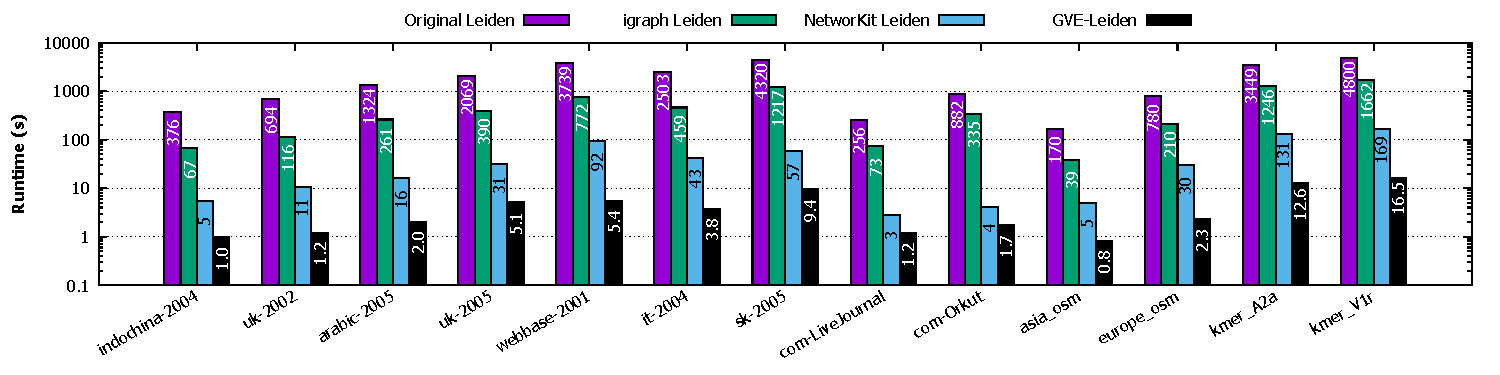
\includegraphics[width=0.98\linewidth]{out/leiden-runtime.pdf}
  } \\[-0ex]
  \subfigure[Speedup of \textit{GVE-Leiden} (logarithmic scale) with respect to \textit{Original Leiden}, \textit{igraph Leiden}, \textit{NetworKit Leiden}.]{
    \label{fig:leiden-compare--speedup}
    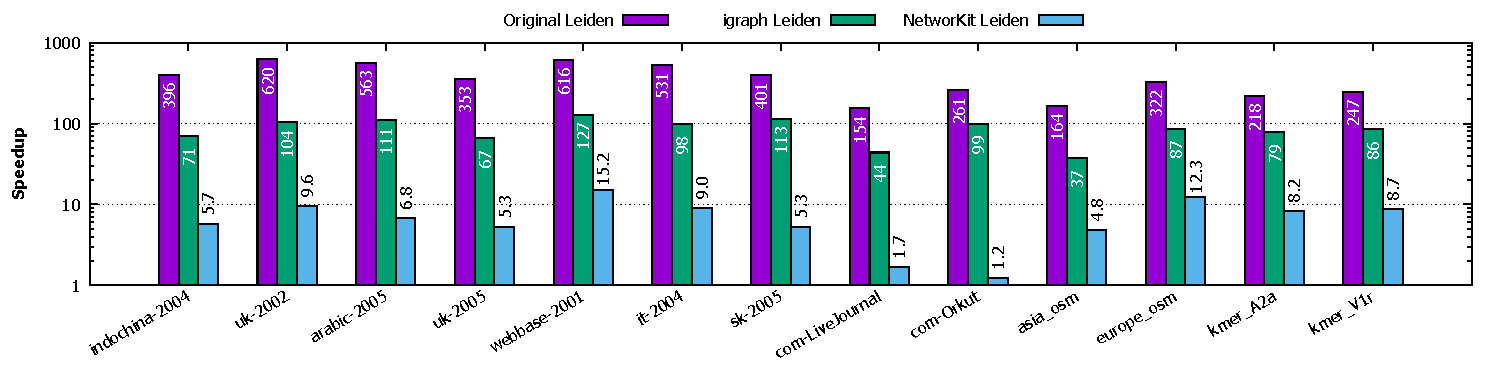
\includegraphics[width=0.98\linewidth]{out/leiden-speedup.pdf}
  } \\[-0ex]
  \subfigure[Modularity of communities obtained with \textit{Original Leiden}, \textit{igraph Leiden}, \textit{NetworKit Leiden}, and \textit{GVE-Leiden}.]{
    \label{fig:leiden-compare--modularity}
    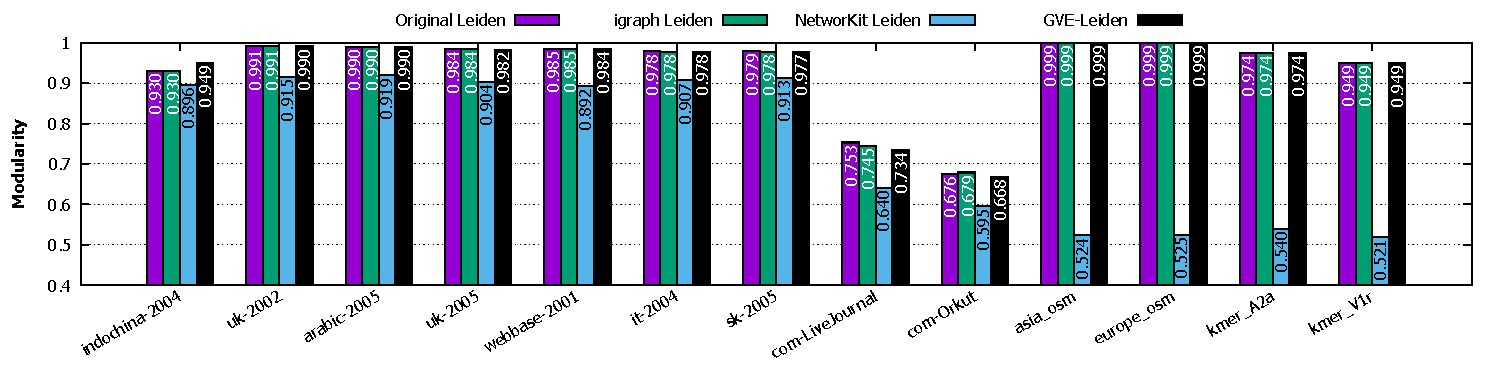
\includegraphics[width=0.98\linewidth]{out/leiden-modularity.pdf}
  } \\[-0ex]
  \subfigure[Fraction of disconnected communities (logarithmic scale) with \textit{Original Leiden}, \textit{igraph Leiden}, \textit{NetworKit Leiden}, and \textit{GVE-Leiden}.]{
    \label{fig:leiden-compare--disconnected}
    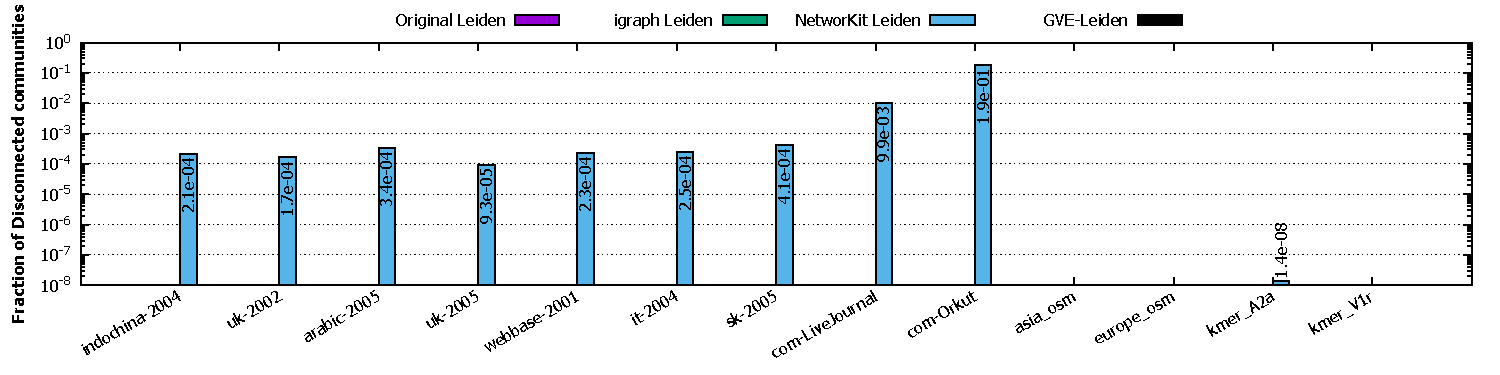
\includegraphics[width=0.98\linewidth]{out/leiden-disconnected.pdf}
  } \\[-2ex]
  \caption{Runtime in seconds (log-scale), speedup (log-scale), modularity, and fraction of disconnected communities (log-scale) with \textit{Original Leiden}, \textit{igraph Leiden}, \textit{NetworKit Leiden}, and \textit{GVE-Leiden} for each graph in the dataset.}
  \label{fig:leiden-compare}
\end{figure*}

\begin{figure*}[hbtp]
  \centering
  \subfigure[Runtime in seconds (logarithmic scale) with \textit{GVE-Louvain} and \textit{GVE-Leiden}]{
    \label{fig:gve-compare--runtime}
    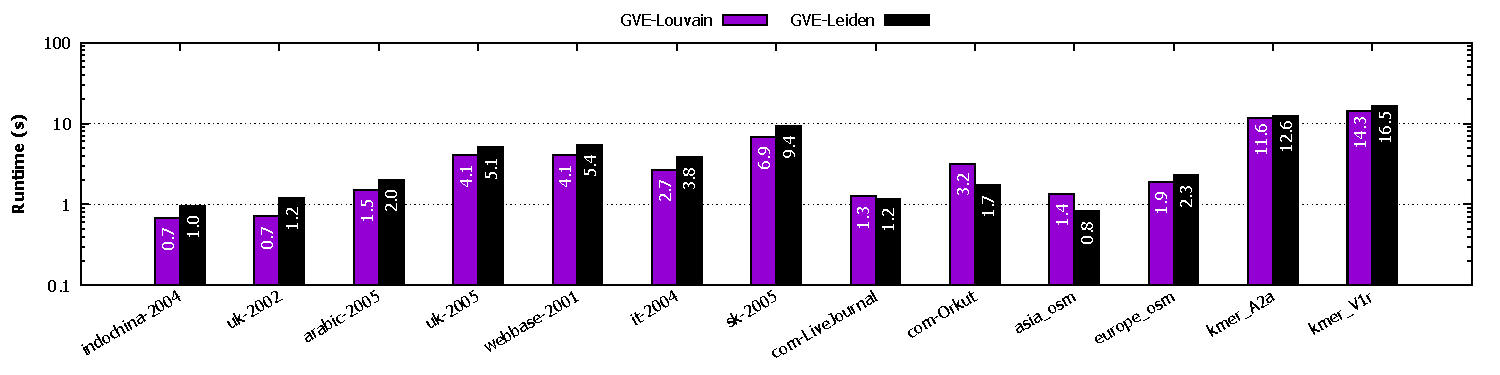
\includegraphics[width=0.98\linewidth]{out/gve-runtime.pdf}
  } \\[-0ex]
  \subfigure[Speedup of \textit{GVE-Leiden} with respect to \textit{GVE-Louvain}. \textit{GVE-Leiden} is generally slower (speedup < $1$) because of additional refinement phase.]{
    \label{fig:gve-compare--speedup}
    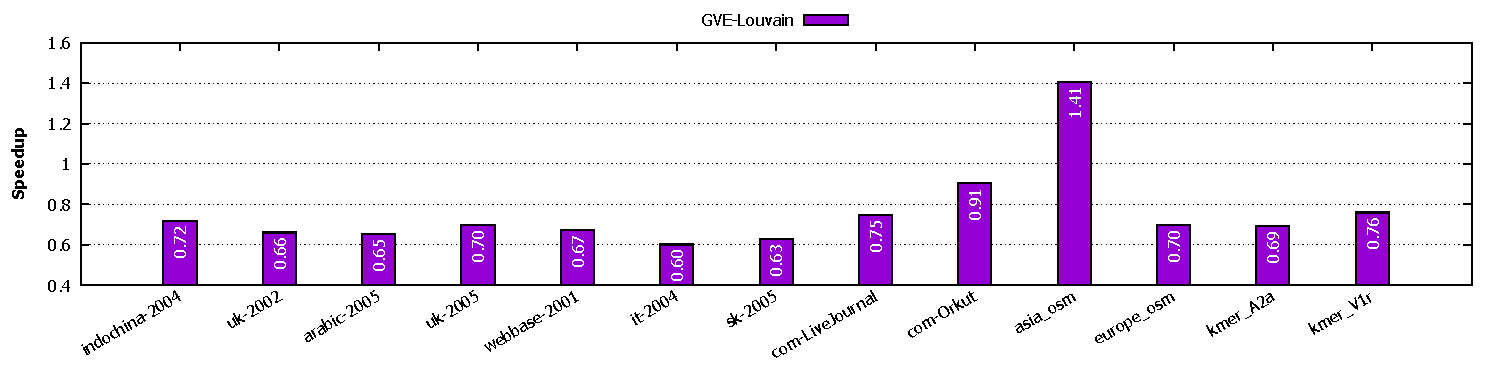
\includegraphics[width=0.98\linewidth]{out/gve-speedup.pdf}
  } \\[-0ex]
  \subfigure[Modularity of communities obtained with \textit{GVE-Louvain} and \textit{GVE-Leiden}.]{
    \label{fig:gve-compare--modularity}
    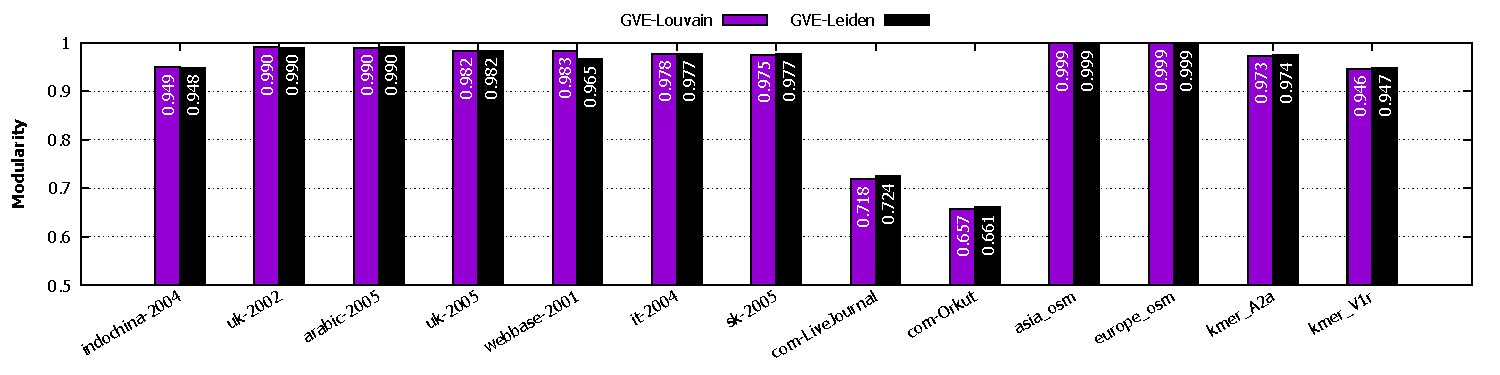
\includegraphics[width=0.98\linewidth]{out/gve-modularity.pdf}
  } \\[-0ex]
  \subfigure[Fraction of disconnected communities (logarithmic scale) with \textit{GVE-Louvain} and \textit{GVE-Leiden}.]{
    \label{fig:gve-compare--disconnected}
    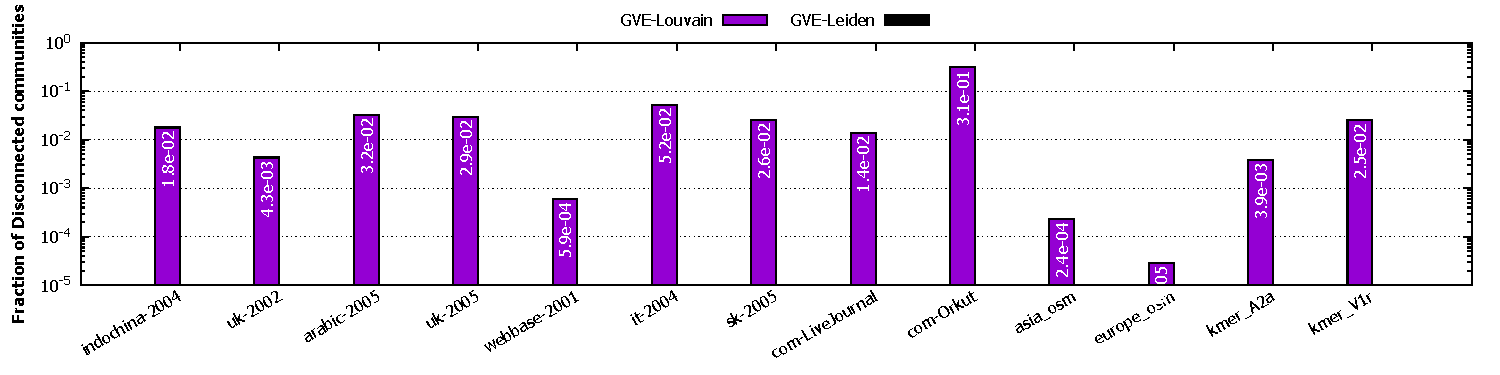
\includegraphics[width=0.98\linewidth]{out/gve-disconnected.pdf}
  } \\[-2ex]
  \caption{Runtime in seconds (log-scale), speedup, modularity, and fraction of disconnected communities (log-scale) with \textit{GVE-Louvain} and \textit{GVE-Leiden} for each graph in the dataset.}
  \label{fig:gve-compare}
\end{figure*}





\subsection{Comparing Performance of GVE-Leiden}

We now compare the performance of GVE-Leiden with the original Leiden \cite{com-traag19}, igraph Leiden \cite{csardi2006igraph}, and NetworKit Leiden \cite{staudt2016networkit}. For the original Leiden, we use a C++ program to initialize a \texttt{ModularityVertexPartition} upon the loaded graph, and invoke \texttt{optimise\_partition()} to obtain the community membership of each vertex in the graph. For igraph Leiden, we use \texttt{igraph\_community\_leiden()} with a resolution of $1/2|E|$, a beta of $0.01$, and request the algorithm to run until convergence. For NetworKit Leiden, we write a Python script to call \texttt{ParallelLeiden().run()}, while limiting the number of passes to $10$. For each graph, we measure the runtime of each implementation five times, for averaging. We also record the modularity of communities obtained, as reported by each implementation, save the community membership vector to a file, and later count the number of disconnected components with Algorithm \ref{alg:disconnected}. In all cases, we use modularity as the quality function to optimize for.

Figure \ref{fig:leiden-compare--runtime} shows the runtimes of the original Leiden, igraph Leiden, NetworKit Leiden, and GVE-Leiden on each graph in the dataset. Figure \ref{fig:leiden-compare--speedup} shows the speedup of GVE-Leiden with respect to each implementation mentioned above. GVE-Leiden is on average $373\times$, $86\times$, and $7.2\times$ faster than the original Leiden, igraph Leiden, and NetworKit Leiden respectively. On the \textit{sk-2005} graph, GVE-Leiden finds communities in $10.8$ seconds, and thus achieve a processing rate of $352$ million edges/s. Figure \ref{fig:leiden-compare--modularity} shows the modularity of communities obtained with each implementation. GVE-Leiden on average obtains $0.1\%$ lower modularity than the original Leiden and igraph Leiden, and $20\%$ higher modularity than NetworKit Leiden (especially on road networks and protein k-mer graphs). Finally, Figure \ref{fig:leiden-compare--disconnected} shows the fraction of disconnected communities obtained with each implementation. Here, absence of bars indicates the absence of disconnected communities. Communities identified by GVE-Leiden on average have $88\times$, $145\times$, and $0.76\times$ disconnected communities than the original Leiden, igraph Leiden, and NetworKit Leiden respectively. While this compares unfavorably with the original Leiden and igraph Leiden, it may be simpler to split the disconnected communities obtained from GVE-Leiden as a post-processing step. We would like to address this issue some time in the future.

Next, we compare the performance of GVE-Leiden with GVE-Louvain \cite{sahu2023gvelouvain}. As above, for each graphs in the dataset, we run both algorithms 5 times to minimize measurement noise, and report the average in Figures \ref{fig:gve-compare--runtime}, \ref{fig:gve-compare--speedup}, \ref{fig:gve-compare--modularity}, and \ref{fig:gve-compare--disconnected}. Figure \ref{fig:gve-compare--runtime} shows the runtimes of GVE-Louvain and GVE-Leiden on each graph in the dataset. Figure \ref{fig:gve-compare--speedup} shows the speedup of GVE-Leiden with respect to GVE-Louvain. GVE-Leiden is on average $24\%$ slower than GVE-Louvain. This increase in computation time is a trade-off for obtaining significantly fewer disconnected communities, as given below. Figure \ref{fig:gve-compare--modularity} shows the modularity of communities obtained with GVE-Louvain and GVE-Leiden. GVE-Leiden on average obtains $0.3\%$ higher modularity than GVE-Louvain. Finally, Figure \ref{fig:gve-compare--disconnected} shows the fraction of disconnected communities obtained with GVE-Louvain and GVE-Leiden. Communities identified by GVE-Leiden on average has an $11$-fold decrease in the number of disconnected communities than GVE-Louvain.

\begin{figure*}[hbtp]
  \centering
  \subfigure[Phase split]{
    \label{fig:leiden-splits--phase}
    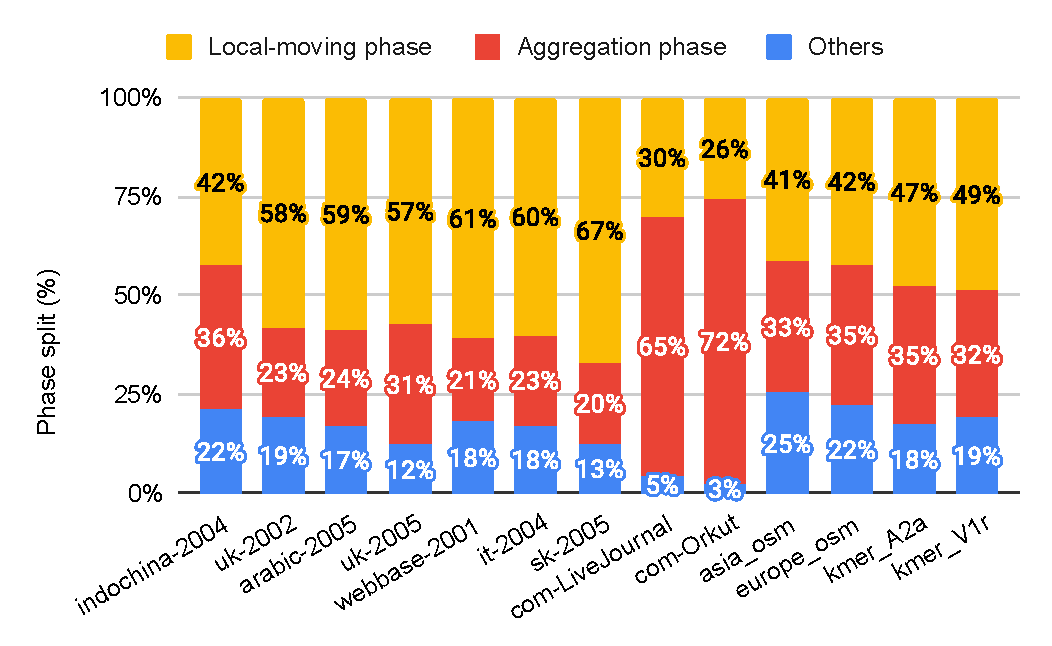
\includegraphics[width=0.48\linewidth]{out/leiden-phases.pdf}
  }
  \subfigure[Pass split]{
    \label{fig:leiden-splits--pass}
    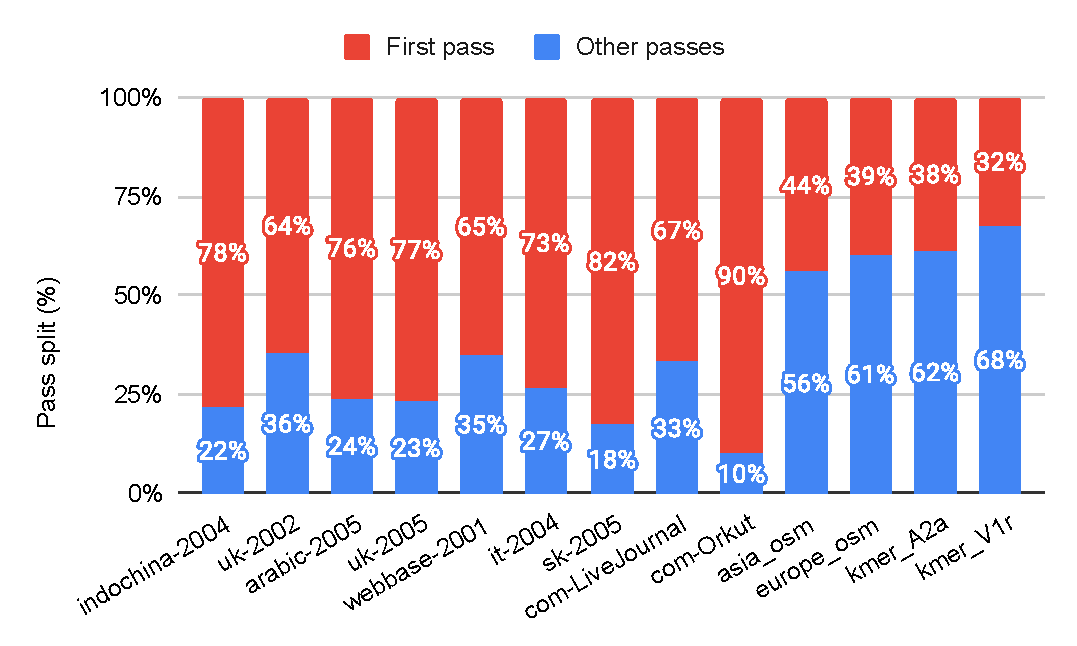
\includegraphics[width=0.48\linewidth]{out/leiden-passes.pdf}
  } \\[-2ex]
  \caption{Phase split of \textit{GVE-Leiden} shown on the left, and pass split shown on the right for each graph in the dataset.}
  \label{fig:leiden-splits}
\end{figure*}

\begin{figure}[hbtp]
  \centering
  \subfigure{
    \label{fig:leiden-hardness--all}
    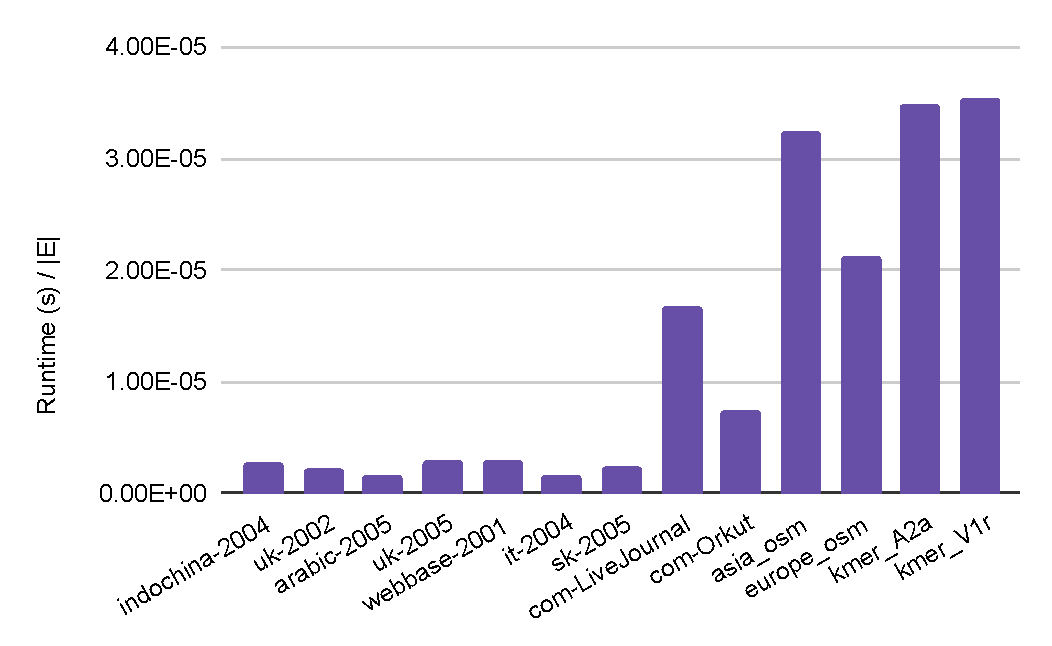
\includegraphics[width=0.98\linewidth]{out/leiden-hardness.pdf}
  } \\[-2ex]
  \caption{Runtime $/ |E|$ factor with \textit{GVE-Leiden} for each graph in the dataset.}
  \label{fig:leiden-hardness}
\end{figure}

\begin{figure}[hbtp]
  \centering
  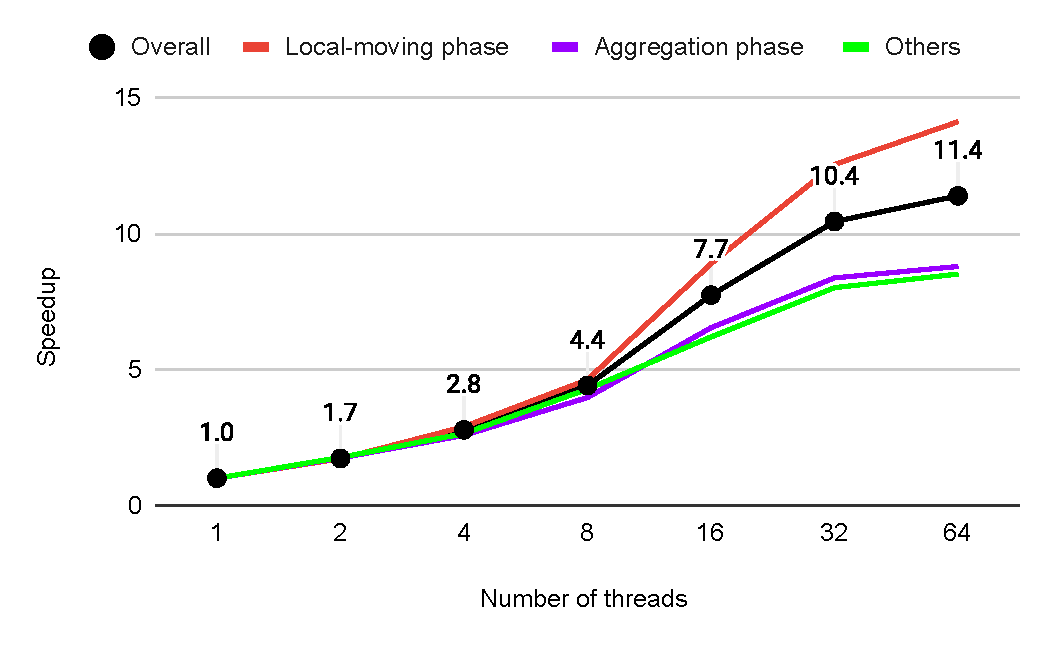
\includegraphics[width=0.98\linewidth]{out/leiden-ss.pdf} \\[-2ex]
  \caption{Overall speedup of \textit{GVE-Leiden}, and its various phases (local-moving, refinement, aggregation, others), with increasing number of threads (in multiples of 2).}
  \label{fig:leiden-ss}
\end{figure}





\subsection{Analyzing Performance of GVE-Leiden}

The phase-wise and pass-wise split of GVE-Leiden is shown in Figures \ref{fig:leiden-splits--phase} and \ref{fig:leiden-splits--pass} respectively. Figure \ref{fig:leiden-splits--phase} indicates that GVE-Leiden spends most of the runtime in the local-moving and refinement phases on \textit{web graphs}, \textit{road networks}, and \textit{protein k-mer graphs}, while it devotes majority of the runtime in the aggregation phase on \textit{social networks}. The pass-wise split (Figure \ref{fig:leiden-splits--pass}) indicates that the first pass dominates runtime on high-degree graphs (\textit{web graphs} and \textit{social networks}), while subsequent passes prevail in execution time on low-degree graphs (\textit{road networks} and \textit{protein k-mer graphs}).

On average, $37\%$ of GVE-Leiden's runtime is spent in the local-moving phase, $27\%$ in the refinement phase, $24\%$ is spent in the aggregation phase, and $12\%$ is spent in other steps (initialization, renumbering communities, looking up dendrogram, and resetting communities) of the algorithm. Further, $73\%$ of the runtime is spent in the first pass of the algorithm, which is the most expensive pass due to the size of the original graph (later passes work on super-vertex graphs).

We also observe that graphs with lower average degree (\textit{road networks} and \textit{protein k-mer graphs}) and graphs with poor community structure (such as \verb|com-LiveJournal| and \verb|com-Orkut|) have a larger $\text{runtime}/|E|$ factor, as shown in Figure \ref{fig:leiden-hardness}.




\subsection{Strong Scaling of GVE-Leiden}

Finally, we measure the strong scaling performance of GVE-Leiden. To this end, we adjust the number of threads from $1$ to $64$ in multiples of $2$ for each input graph, and measure the overall time taken for finding communities with GVE-Leiden, as well as its phase splits (local-moving, refinement, aggregation, others), five times for averaging. The results are shown in Figure \ref{fig:leiden-ss}. With 32 threads, GVE-Leiden obtains an average speedup of $10.9\times$ compared to running with a single thread, i.e., its performance increases by $1.6\times$ for every doubling of threads. Scaling is limited due to the various sequential steps/phases in the algorithm. At 64 threads, GVE-Leiden is impacted by NUMA effects, and offers speedup of only $12.9\times$.


\section{Conclusion}
\label{sec:conclusion}
In conclusion, this study addresses the design of an optimized parallel implementation of the Leiden algorithm \cite{com-traag19}, a high-quality community detection algorithm that improves upon the popular Louvain method \cite{com-blondel08}, in the shared memory setting. We extend optimizations for the Louvain algorithm \cite{sahu2023gvelouvain} to our implementation of the Leiden algorithm, and use a greedy refinement phase where vertices greedily optimize for delta-modularity within their community bounds, which we observe, offers both better performance and quality than a randomized approach.

On a system equipped with two 16-core Intel Xeon Gold 6226R processors, our implementation of the Leiden algorithm, referred to as GVE-Leiden, attains a processing rate of $352 M$ edges per second on a $3.8 B$ edge graph. It surpasses the original Leiden implementation, igraph Leiden, and NetworKit Leiden by factors of $373\times$, $86\times$, and $7.2\times$ respectively. GVE-Leiden identifies communities of equivalent quality to the first two implementations, and $26\%$ higher quality than NetworKit. Doubling the number of threads results in an average performance scaling of $1.6\times$ for GVE-Leiden. In comparison to GVE-Louvain \cite{sahu2023gvelouvain}, our parallel Louvain implementation, GVE-Leiden reduces internally-disconnected communities by a factor of $11$ with only a $36\%$ increase in runtime.

However, on average, communities identified by GVE-Leiden exhibit $88\times$, $145\times$, and $0.76\times$ more disconnected communities compared to the original Leiden, igraph Leiden, and NetworKit Leiden, respectively. This disparity is particularly noticeable on \textit{social networks}, \textit{road networks}, and \textit{protein k-mer graphs}. Despite this drawback, a potential solution is to address the issue by post-processing, where disconnected communities obtained from GVE-Leiden can be split. We acknowledge this concern, and plan to explore solutions in future work.


%% The acknowledgments section.
\begin{acks}
I would like to thank Prof. Kishore Kothapalli, Prof. Dip Sankar Banerjee, Vincent Traag, Geerten Verweij, Fabian Nguyen, Chuck Hastings, and Rick Ratzel for their support.
\end{acks}

%% Bibliography style to be used, and the bibliography file.
\bibliographystyle{ACM-Reference-Format}
\bibliography{main}

\clearpage
\appendix
\section{Appendix}

\subsection{Community labels of super-vertices}

We also attempt two different variations of Parallel Leiden algorithm, one where the community labels of super-vertices (upon aggregation) is based on the local-moving phase (\textit{move-based}), and the other where the community labels of super-vertices is based on the refinement phase (\textit{refine-based}). Our observations indicate that both approaches have roughly the same runtime and modularity on average, as indicated by Figures \ref{fig:leidenreopt-runtime} and \ref{fig:leidenreopt-modularity}. Accordingly, we stick to the move-based approach, which is the one recommended by Traag et al. \cite{com-traag19}. However, the refine-based may be more suitable for the design of dynamic Leiden algorithm (for dynamic graphs).

\begin{figure}[hbtp]
  \centering
  \subfigure{
    \label{fig:leidenreopt-runtime--all}
    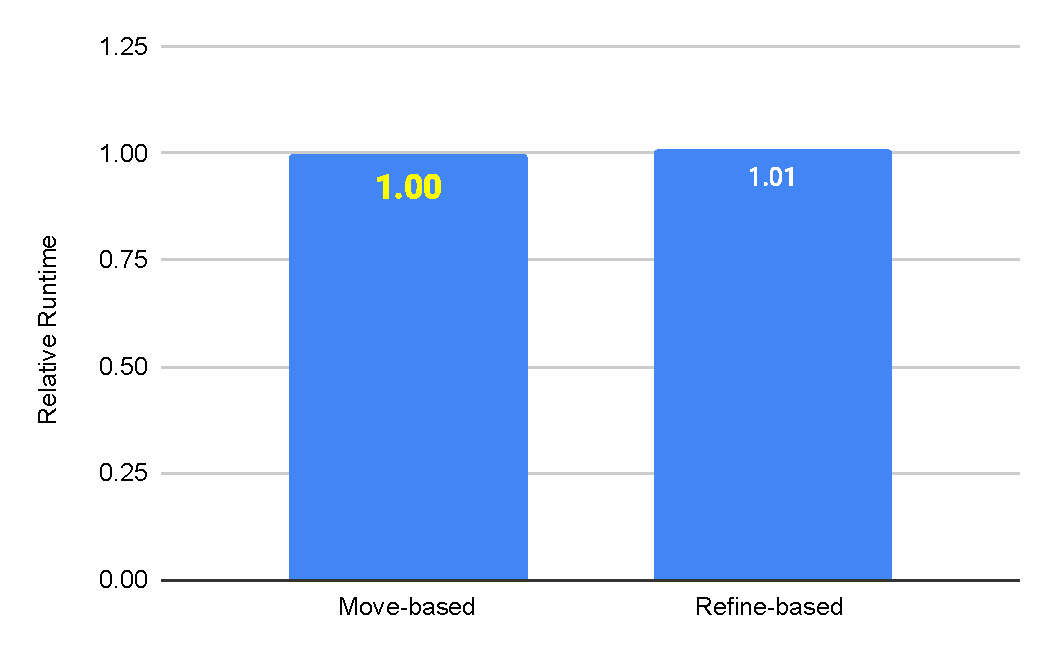
\includegraphics[width=0.98\linewidth]{out/leidenreopt-runtime.pdf}
  } \\[-2ex]
  \caption{Average relative runtime for \textit{move-based} and \textit{refine-based} communities for super-vertices upon aggregation with parallel Leiden algorithm, for all graphs in the dataset.}
  \label{fig:leidenreopt-runtime}
\end{figure}

\begin{figure}[hbtp]
  \centering
  \subfigure{
    \label{fig:leidenreopt-modularity--all}
    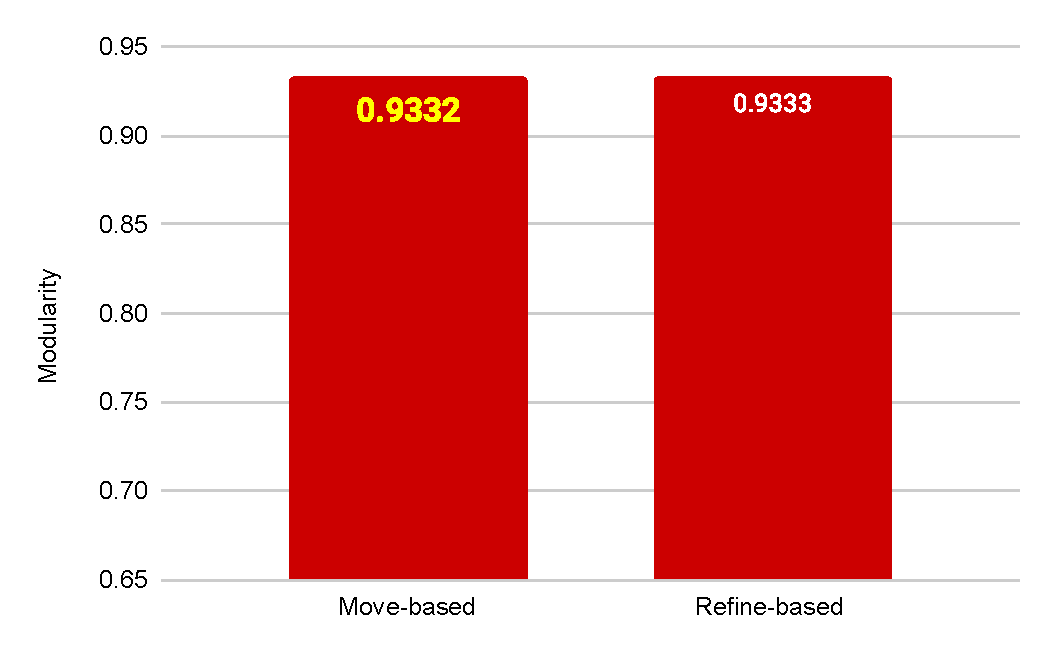
\includegraphics[width=0.98\linewidth]{out/leidenreopt-modularity.pdf}
  } \\[-2ex]
  \caption{Average modularity for \textit{move-based} and \textit{refine-based} communities for super-vertices upon aggregation with parallel Leiden algorithm, for all graphs in the dataset.}
  \label{fig:leidenreopt-modularity}
\end{figure}


\end{document}
\endinput
%% End of file.
